% Options for packages loaded elsewhere
\PassOptionsToPackage{unicode}{hyperref}
\PassOptionsToPackage{hyphens}{url}
\documentclass[
]{book}
\usepackage{xcolor}
\usepackage{amsmath,amssymb}
\setcounter{secnumdepth}{5}
\usepackage{iftex}
\ifPDFTeX
  \usepackage[T1]{fontenc}
  \usepackage[utf8]{inputenc}
  \usepackage{textcomp} % provide euro and other symbols
\else % if luatex or xetex
  \usepackage{unicode-math} % this also loads fontspec
  \defaultfontfeatures{Scale=MatchLowercase}
  \defaultfontfeatures[\rmfamily]{Ligatures=TeX,Scale=1}
\fi
\usepackage{lmodern}
\ifPDFTeX\else
  % xetex/luatex font selection
\fi
% Use upquote if available, for straight quotes in verbatim environments
\IfFileExists{upquote.sty}{\usepackage{upquote}}{}
\IfFileExists{microtype.sty}{% use microtype if available
  \usepackage[]{microtype}
  \UseMicrotypeSet[protrusion]{basicmath} % disable protrusion for tt fonts
}{}
\makeatletter
\@ifundefined{KOMAClassName}{% if non-KOMA class
  \IfFileExists{parskip.sty}{%
    \usepackage{parskip}
  }{% else
    \setlength{\parindent}{0pt}
    \setlength{\parskip}{6pt plus 2pt minus 1pt}}
}{% if KOMA class
  \KOMAoptions{parskip=half}}
\makeatother
\usepackage{color}
\usepackage{fancyvrb}
\newcommand{\VerbBar}{|}
\newcommand{\VERB}{\Verb[commandchars=\\\{\}]}
\DefineVerbatimEnvironment{Highlighting}{Verbatim}{commandchars=\\\{\}}
% Add ',fontsize=\small' for more characters per line
\usepackage{framed}
\definecolor{shadecolor}{RGB}{248,248,248}
\newenvironment{Shaded}{\begin{snugshade}}{\end{snugshade}}
\newcommand{\AlertTok}[1]{\textcolor[rgb]{0.94,0.16,0.16}{#1}}
\newcommand{\AnnotationTok}[1]{\textcolor[rgb]{0.56,0.35,0.01}{\textbf{\textit{#1}}}}
\newcommand{\AttributeTok}[1]{\textcolor[rgb]{0.13,0.29,0.53}{#1}}
\newcommand{\BaseNTok}[1]{\textcolor[rgb]{0.00,0.00,0.81}{#1}}
\newcommand{\BuiltInTok}[1]{#1}
\newcommand{\CharTok}[1]{\textcolor[rgb]{0.31,0.60,0.02}{#1}}
\newcommand{\CommentTok}[1]{\textcolor[rgb]{0.56,0.35,0.01}{\textit{#1}}}
\newcommand{\CommentVarTok}[1]{\textcolor[rgb]{0.56,0.35,0.01}{\textbf{\textit{#1}}}}
\newcommand{\ConstantTok}[1]{\textcolor[rgb]{0.56,0.35,0.01}{#1}}
\newcommand{\ControlFlowTok}[1]{\textcolor[rgb]{0.13,0.29,0.53}{\textbf{#1}}}
\newcommand{\DataTypeTok}[1]{\textcolor[rgb]{0.13,0.29,0.53}{#1}}
\newcommand{\DecValTok}[1]{\textcolor[rgb]{0.00,0.00,0.81}{#1}}
\newcommand{\DocumentationTok}[1]{\textcolor[rgb]{0.56,0.35,0.01}{\textbf{\textit{#1}}}}
\newcommand{\ErrorTok}[1]{\textcolor[rgb]{0.64,0.00,0.00}{\textbf{#1}}}
\newcommand{\ExtensionTok}[1]{#1}
\newcommand{\FloatTok}[1]{\textcolor[rgb]{0.00,0.00,0.81}{#1}}
\newcommand{\FunctionTok}[1]{\textcolor[rgb]{0.13,0.29,0.53}{\textbf{#1}}}
\newcommand{\ImportTok}[1]{#1}
\newcommand{\InformationTok}[1]{\textcolor[rgb]{0.56,0.35,0.01}{\textbf{\textit{#1}}}}
\newcommand{\KeywordTok}[1]{\textcolor[rgb]{0.13,0.29,0.53}{\textbf{#1}}}
\newcommand{\NormalTok}[1]{#1}
\newcommand{\OperatorTok}[1]{\textcolor[rgb]{0.81,0.36,0.00}{\textbf{#1}}}
\newcommand{\OtherTok}[1]{\textcolor[rgb]{0.56,0.35,0.01}{#1}}
\newcommand{\PreprocessorTok}[1]{\textcolor[rgb]{0.56,0.35,0.01}{\textit{#1}}}
\newcommand{\RegionMarkerTok}[1]{#1}
\newcommand{\SpecialCharTok}[1]{\textcolor[rgb]{0.81,0.36,0.00}{\textbf{#1}}}
\newcommand{\SpecialStringTok}[1]{\textcolor[rgb]{0.31,0.60,0.02}{#1}}
\newcommand{\StringTok}[1]{\textcolor[rgb]{0.31,0.60,0.02}{#1}}
\newcommand{\VariableTok}[1]{\textcolor[rgb]{0.00,0.00,0.00}{#1}}
\newcommand{\VerbatimStringTok}[1]{\textcolor[rgb]{0.31,0.60,0.02}{#1}}
\newcommand{\WarningTok}[1]{\textcolor[rgb]{0.56,0.35,0.01}{\textbf{\textit{#1}}}}
\usepackage{longtable,booktabs,array}
\usepackage{calc} % for calculating minipage widths
% Correct order of tables after \paragraph or \subparagraph
\usepackage{etoolbox}
\makeatletter
\patchcmd\longtable{\par}{\if@noskipsec\mbox{}\fi\par}{}{}
\makeatother
% Allow footnotes in longtable head/foot
\IfFileExists{footnotehyper.sty}{\usepackage{footnotehyper}}{\usepackage{footnote}}
\makesavenoteenv{longtable}
\usepackage{graphicx}
\makeatletter
\newsavebox\pandoc@box
\newcommand*\pandocbounded[1]{% scales image to fit in text height/width
  \sbox\pandoc@box{#1}%
  \Gscale@div\@tempa{\textheight}{\dimexpr\ht\pandoc@box+\dp\pandoc@box\relax}%
  \Gscale@div\@tempb{\linewidth}{\wd\pandoc@box}%
  \ifdim\@tempb\p@<\@tempa\p@\let\@tempa\@tempb\fi% select the smaller of both
  \ifdim\@tempa\p@<\p@\scalebox{\@tempa}{\usebox\pandoc@box}%
  \else\usebox{\pandoc@box}%
  \fi%
}
% Set default figure placement to htbp
\def\fps@figure{htbp}
\makeatother
\setlength{\emergencystretch}{3em} % prevent overfull lines
\providecommand{\tightlist}{%
  \setlength{\itemsep}{0pt}\setlength{\parskip}{0pt}}
\usepackage[]{natbib}
\bibliographystyle{plainnat}
\usepackage{booktabs}
\usepackage{bookmark}
\IfFileExists{xurl.sty}{\usepackage{xurl}}{} % add URL line breaks if available
\urlstyle{same}
\hypersetup{
  pdftitle={Times Series Part II},
  pdfauthor={Samuel Rowe adapted from Wooldridge (2011)},
  hidelinks,
  pdfcreator={LaTeX via pandoc}}

\title{Times Series Part II}
\author{Samuel Rowe adapted from Wooldridge (2011)}
\date{2025-09-19}

\begin{document}
\maketitle

{
\setcounter{tocdepth}{1}
\tableofcontents
}
\begin{Shaded}
\begin{Highlighting}[]
\NormalTok{bookdown}\SpecialCharTok{::}\FunctionTok{render\_book}\NormalTok{()}
\end{Highlighting}
\end{Shaded}

\chapter*{Overview}\label{overview}
\addcontentsline{toc}{chapter}{Overview}

Topics for Week 12:

\begin{enumerate}
\def\labelenumi{\arabic{enumi}.}
\tightlist
\item
  Unit Roots
\item
  Testing for Serial Correlation
\item
  Correcting for Serial Correlation
\end{enumerate}

\chapter{Unit Roots}\label{unit-roots}

\textbf{Lesson:} when we have a unit root process or Time Series integrated of order one \(I(1)\)
we can use a first difference to transform the time series into a weakly dependent
and often stationary process.

\section{Example: Revisit Fertility}\label{example-revisit-fertility}

Set the time series

\begin{Shaded}
\begin{Highlighting}[]
\NormalTok{cd }\StringTok{"/Users/Sam/Desktop/Econ 645/Data/Wooldridge"}
\KeywordTok{use}\NormalTok{ fertil3.dta, }\KeywordTok{clear}
\KeywordTok{tsset} \FunctionTok{year}
\end{Highlighting}
\end{Shaded}

\begin{verbatim}
/Users/Sam/Desktop/Econ 645/Data/Wooldridge

        time variable:  year, 1913 to 1984
                delta:  1 unit
\end{verbatim}

Plot the Graph

\begin{Shaded}
\begin{Highlighting}[]
\KeywordTok{twoway} \KeywordTok{line}\NormalTok{ gfr }\FunctionTok{year}\NormalTok{, }\BaseNTok{title}\NormalTok{(}\StringTok{"General Fertility Rate"}\NormalTok{) }\BaseNTok{ytitle}\NormalTok{(}\StringTok{"Children Born per 1,000 CBA Women"}\NormalTok{) }\BaseNTok{xtitle}\NormalTok{(}\StringTok{"Year"}\NormalTok{)}
\KeywordTok{graph} \KeywordTok{export} \StringTok{"/Users/Sam/Desktop/Econ 645/Stata/week\_11\_i1.png"}\NormalTok{, }\KeywordTok{replace}
\end{Highlighting}
\end{Shaded}

\begin{figure}
\centering
\pandocbounded{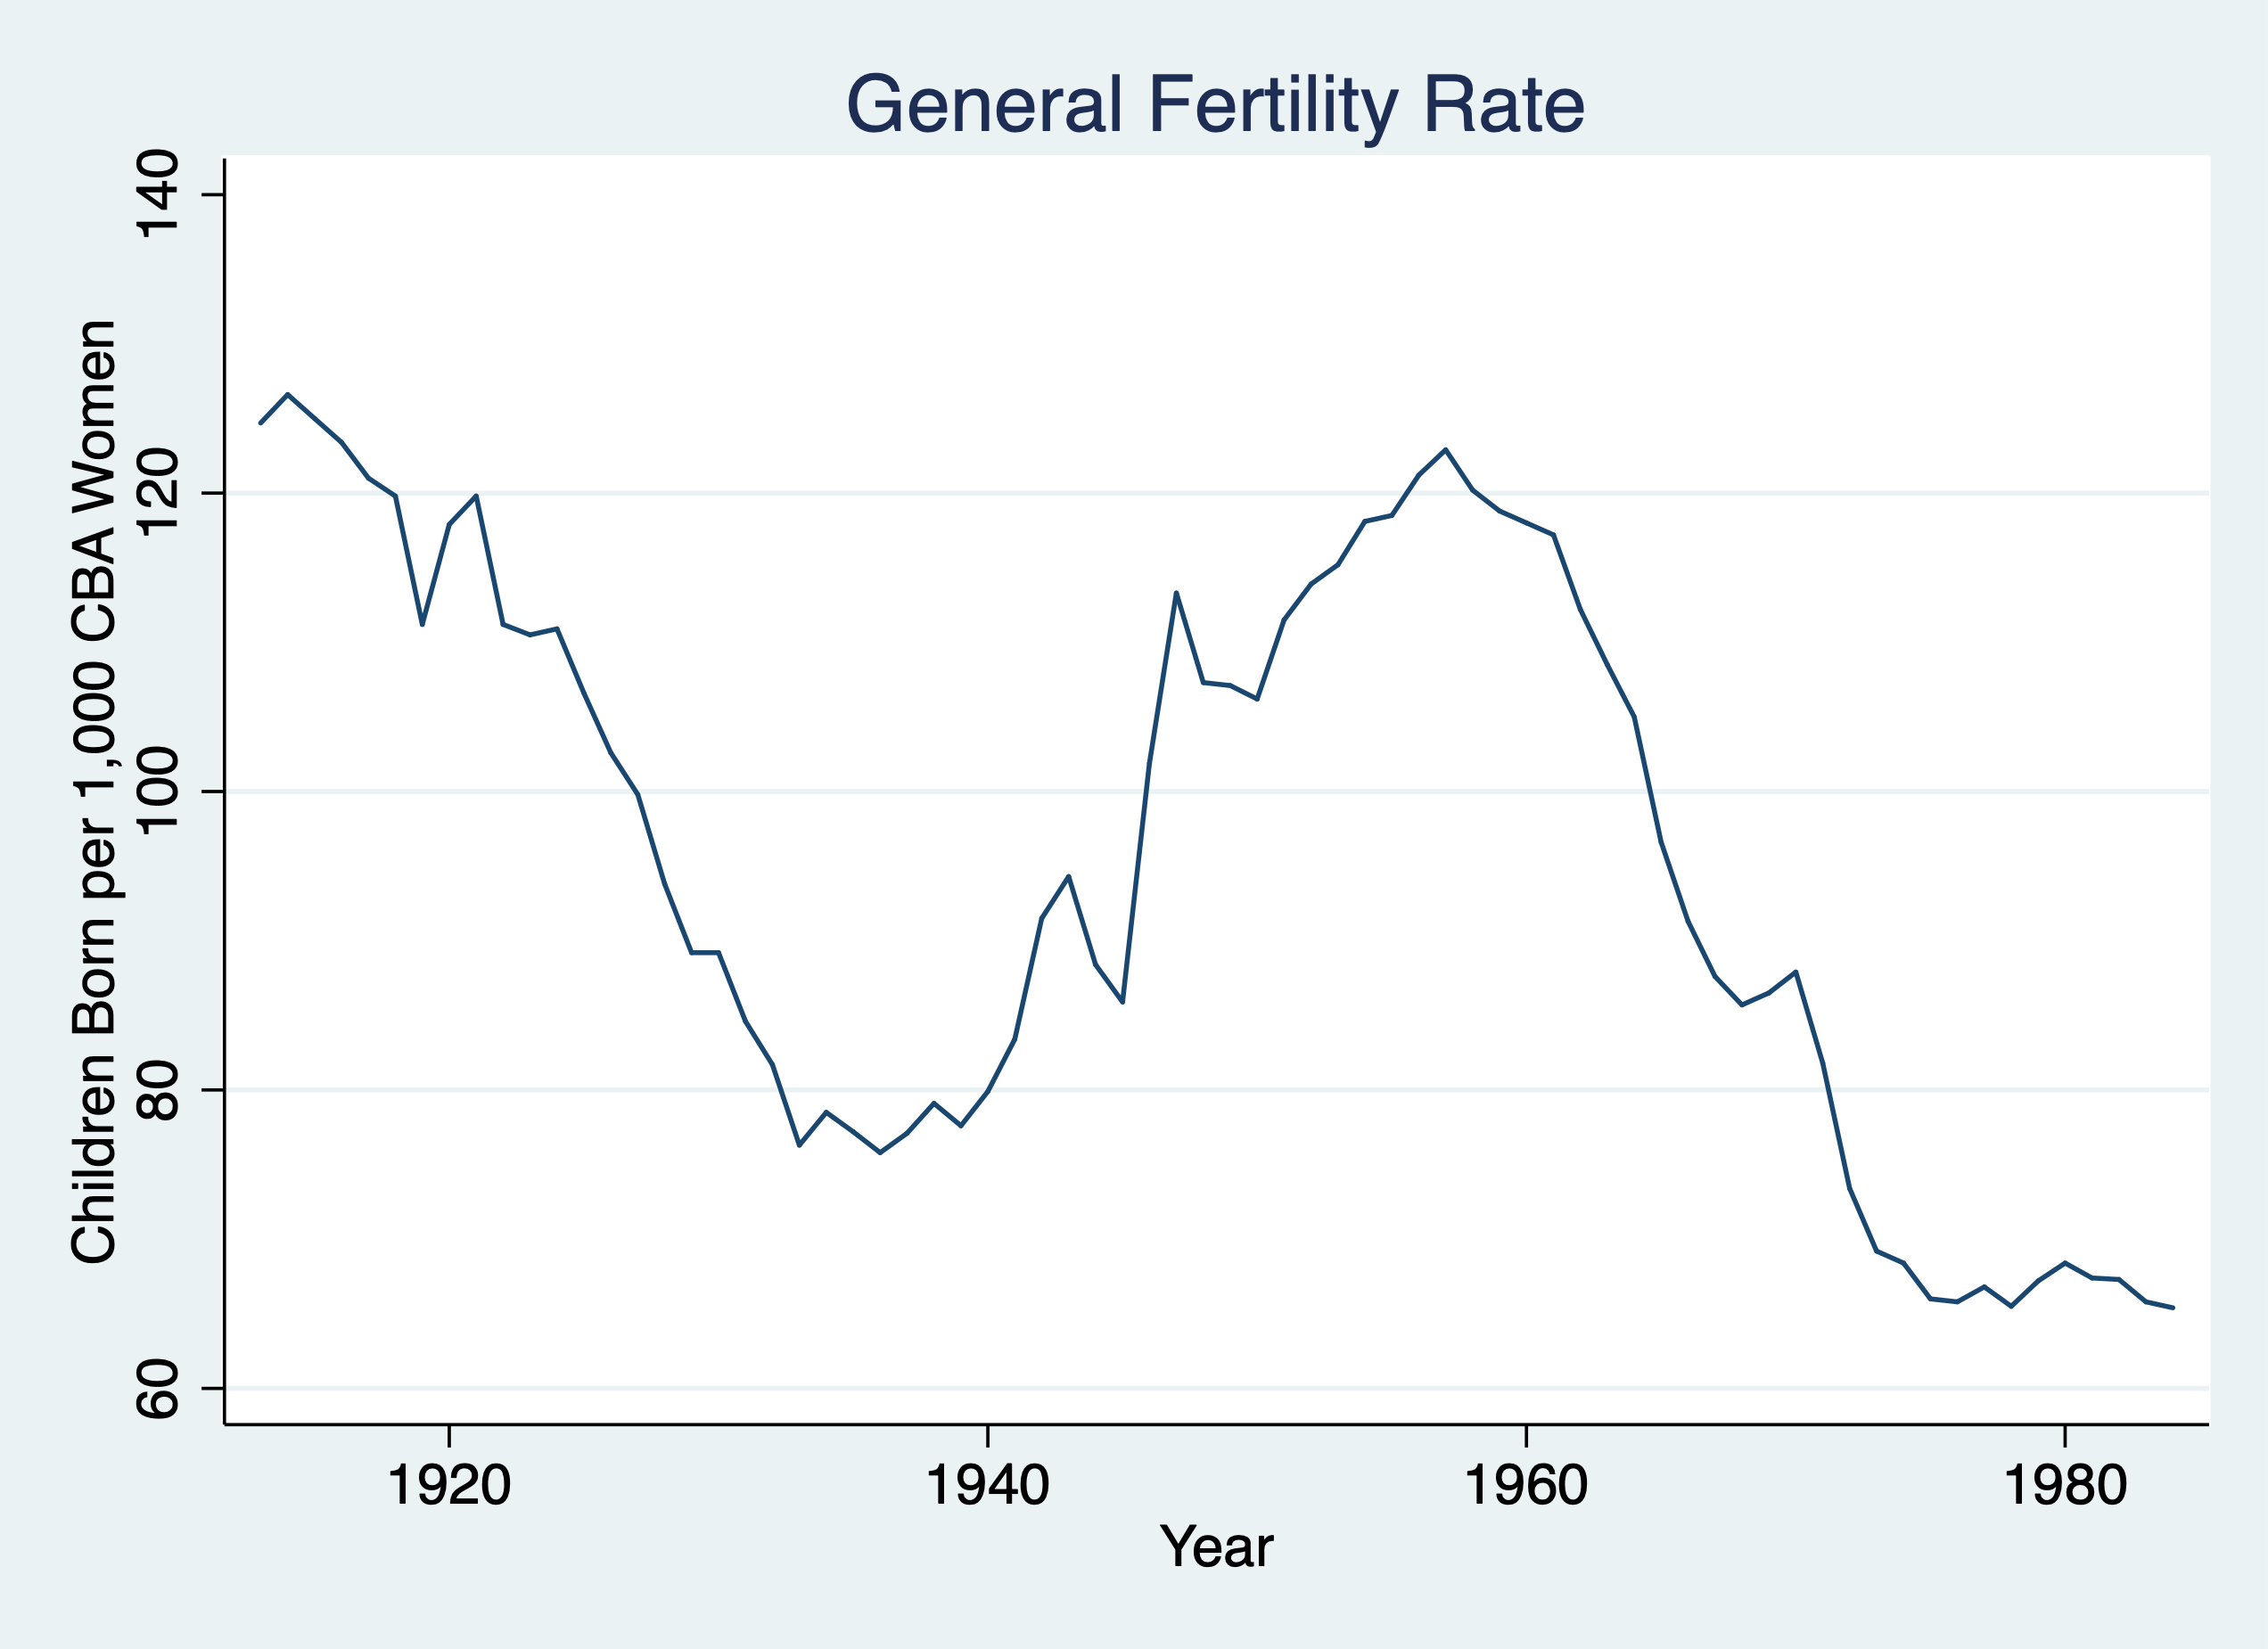
\includegraphics[keepaspectratio]{week_11_i1.png}}
\caption{General Fertility Rate}
\end{figure}

Estimate autocorrelation or estimate \(\hat{\rho}\)

\begin{Shaded}
\begin{Highlighting}[]
\KeywordTok{reg}\NormalTok{ gfr }\OtherTok{l}\NormalTok{.gfr}
\end{Highlighting}
\end{Shaded}

\begin{verbatim}
      Source |       SS           df       MS      Number of obs   =        71
-------------+----------------------------------   F(1, 69)        =   1413.53
       Model |   25734.824         1   25734.824   Prob > F        =    0.0000
    Residual |  1256.21904        69  18.2060731   R-squared       =    0.9535
-------------+----------------------------------   Adj R-squared   =    0.9528
       Total |   26991.043        70  385.586329   Root MSE        =    4.2669

------------------------------------------------------------------------------
         gfr |      Coef.   Std. Err.      t    P>|t|     [95% Conf. Interval]
-------------+----------------------------------------------------------------
         gfr |
         L1. |   .9777202   .0260053    37.60   0.000      .925841    1.029599
             |
       _cons |   1.304937   2.548821     0.51   0.610    -3.779822    6.389695
------------------------------------------------------------------------------
\end{verbatim}

Our result is rho-hat is 0.98, which is indicative of a unit root process.
Under our TS assumptions our t statistics are invalid, but if we use a
transformation using a first-difference process, we can relax those assumptions
under the TSC assumptions. If our \(I(1)\) becomes \(I(0)\), then our TSC assumptions
are potentially valid.

First Difference both dependent and independent

\begin{Shaded}
\begin{Highlighting}[]
\KeywordTok{reg} \KeywordTok{d}\NormalTok{.gfr }\KeywordTok{d}\NormalTok{.pe }\KeywordTok{if} \FunctionTok{year}\NormalTok{ \textless{} 1985}
\end{Highlighting}
\end{Shaded}

\begin{verbatim}
      Source |       SS           df       MS      Number of obs   =        71
-------------+----------------------------------   F(1, 69)        =      2.26
       Model |  40.3237206         1  40.3237206   Prob > F        =    0.1370
    Residual |  1229.25866        69  17.8153428   R-squared       =    0.0318
-------------+----------------------------------   Adj R-squared   =    0.0177
       Total |  1269.58238        70  18.1368911   Root MSE        =    4.2208

------------------------------------------------------------------------------
       D.gfr |      Coef.   Std. Err.      t    P>|t|     [95% Conf. Interval]
-------------+----------------------------------------------------------------
          pe |
         D1. |  -.0426776   .0283672    -1.50   0.137    -.0992686    .0139134
             |
       _cons |  -.7847796   .5020398    -1.56   0.123    -1.786322    .2167625
------------------------------------------------------------------------------
\end{verbatim}

Our result is that the real value of the personal exemption is associated with
a 0.043 decrease in fertility or a 23 dollar increase in the real value of the
personal exemption is associated with a 1 child per capita (1,000 CBA Women).
This is a bit unexpected, but still insignificant. Let's add some lags.

First differnce with more than 1 lag

\begin{Shaded}
\begin{Highlighting}[]
\KeywordTok{reg} \KeywordTok{d}\NormalTok{.gfr }\KeywordTok{d}\NormalTok{.pe }\KeywordTok{d}\NormalTok{.pe\_1 }\KeywordTok{d}\NormalTok{.pe\_2 }\KeywordTok{if} \FunctionTok{year}\NormalTok{ \textless{} 1985}
\end{Highlighting}
\end{Shaded}

\begin{verbatim}
      Source |       SS           df       MS      Number of obs   =        69
-------------+----------------------------------   F(3, 65)        =      6.56
       Model |  293.259859         3  97.7532864   Prob > F        =    0.0006
    Residual |  968.199959        65   14.895384   R-squared       =    0.2325
-------------+----------------------------------   Adj R-squared   =    0.1971
       Total |  1261.45982        68  18.5508797   Root MSE        =    3.8595

------------------------------------------------------------------------------
       D.gfr |      Coef.   Std. Err.      t    P>|t|     [95% Conf. Interval]
-------------+----------------------------------------------------------------
          pe |
         D1. |  -.0362021   .0267737    -1.35   0.181     -.089673    .0172687
             |
        pe_1 |
         D1. |  -.0139706   .0275539    -0.51   0.614    -.0689997    .0410584
             |
        pe_2 |
         D1. |   .1099896   .0268797     4.09   0.000     .0563071    .1636721
             |
       _cons |  -.9636787   .4677599    -2.06   0.043     -1.89786   -.0294976
------------------------------------------------------------------------------
\end{verbatim}

Our results show that increases in the current and prior period real value
personal exemption is not statistically significant. However, a 1 dollar increase
in the real value of personal exemption is associated two period prior is associated
with an increase of .110 child per capita (or \$9.1 increase is associated with
an increase of 1 child per capita.

\section{Wages and Productivity}\label{wages-and-productivity}

\(I(1)\) process with the presence of a linear trend

We want to estimate the elasticity of hourly wage with respect to output per hour
(or labor productivity).

\[ ln(hrwage_t)=\beta_0 + \beta_1 ln(outphr_t) + \beta_2 t + u_t \]

Set Time Series and estimate the contemporaneous model

\begin{Shaded}
\begin{Highlighting}[]
\NormalTok{cd }\StringTok{"/Users/Sam/Desktop/Econ 645/Data/Wooldridge"}
\KeywordTok{use}\NormalTok{ earns.dta, }\KeywordTok{clear}
\KeywordTok{tsset} \FunctionTok{year}\NormalTok{, }\FunctionTok{yearly}
\KeywordTok{reg}\NormalTok{ lhrwage loutphr t}
\end{Highlighting}
\end{Shaded}

\begin{verbatim}
/Users/Sam/Desktop/Econ 645/Data/Wooldridge

        time variable:  year, 1947 to 1987
                delta:  1 year

      Source |       SS           df       MS      Number of obs   =        41
-------------+----------------------------------   F(2, 38)        =    641.22
       Model |  1.04458064         2  .522290318   Prob > F        =    0.0000
    Residual |  .030951776        38   .00081452   R-squared       =    0.9712
-------------+----------------------------------   Adj R-squared   =    0.9697
       Total |  1.07553241        40   .02688831   Root MSE        =    .02854

------------------------------------------------------------------------------
     lhrwage |      Coef.   Std. Err.      t    P>|t|     [95% Conf. Interval]
-------------+----------------------------------------------------------------
     loutphr |   1.639639   .0933471    17.56   0.000     1.450668    1.828611
           t |    -.01823   .0017482   -10.43   0.000     -.021769   -.0146909
       _cons |  -5.328454   .3744492   -14.23   0.000    -6.086487   -4.570421
------------------------------------------------------------------------------
\end{verbatim}

We estimate that the elasticity is very large, where a 1\% increase in labor
productivity (output per hour) is associated with a 1.64\% increase in hourly
wage. Let's test for autocorrelation with accounting for the linear trend.

\begin{Shaded}
\begin{Highlighting}[]
\KeywordTok{reg}\NormalTok{ lhrwage }\OtherTok{l}\NormalTok{.lhrwage t}
\end{Highlighting}
\end{Shaded}

\begin{verbatim}
      Source |       SS           df       MS      Number of obs   =        40
-------------+----------------------------------   F(2, 37)        =   1595.37
       Model |  .921760671         2  .460880336   Prob > F        =    0.0000
    Residual |  .010688817        37  .000288887   R-squared       =    0.9885
-------------+----------------------------------   Adj R-squared   =    0.9879
       Total |  .932449488        39  .023908961   Root MSE        =      .017

------------------------------------------------------------------------------
     lhrwage |      Coef.   Std. Err.      t    P>|t|     [95% Conf. Interval]
-------------+----------------------------------------------------------------
     lhrwage |
         L1. |   .9842872   .0334331    29.44   0.000     .9165452    1.052029
             |
           t |  -.0009039   .0004732    -1.91   0.064    -.0018626    .0000548
       _cons |   .0544169   .0413998     1.31   0.197    -.0294671    .1383008
------------------------------------------------------------------------------
\end{verbatim}

We have some evidence for a unit root process, so we'll use the first-difference
to transform the I(1) process into a I(0) process. We'll no longer need the
time trend

\begin{Shaded}
\begin{Highlighting}[]
    \KeywordTok{twoway} \KeywordTok{line}\NormalTok{ lhrwage }\FunctionTok{year}\NormalTok{, }\BaseNTok{title}\NormalTok{(}\StringTok{"Natural Log of Hourly Wages"}\NormalTok{) }\BaseNTok{ytitle}\NormalTok{(}\StringTok{"Ln(Hourly Wage)"}\NormalTok{) }\BaseNTok{xtitle}\NormalTok{(}\StringTok{"Year"}\NormalTok{)}
    \KeywordTok{graph} \KeywordTok{export} \StringTok{"/Users/Sam/Desktop/Econ 645/Stata/week\_11\_hrwage1.png"}\NormalTok{, }\KeywordTok{replace}
\end{Highlighting}
\end{Shaded}

\begin{figure}
\centering
\pandocbounded{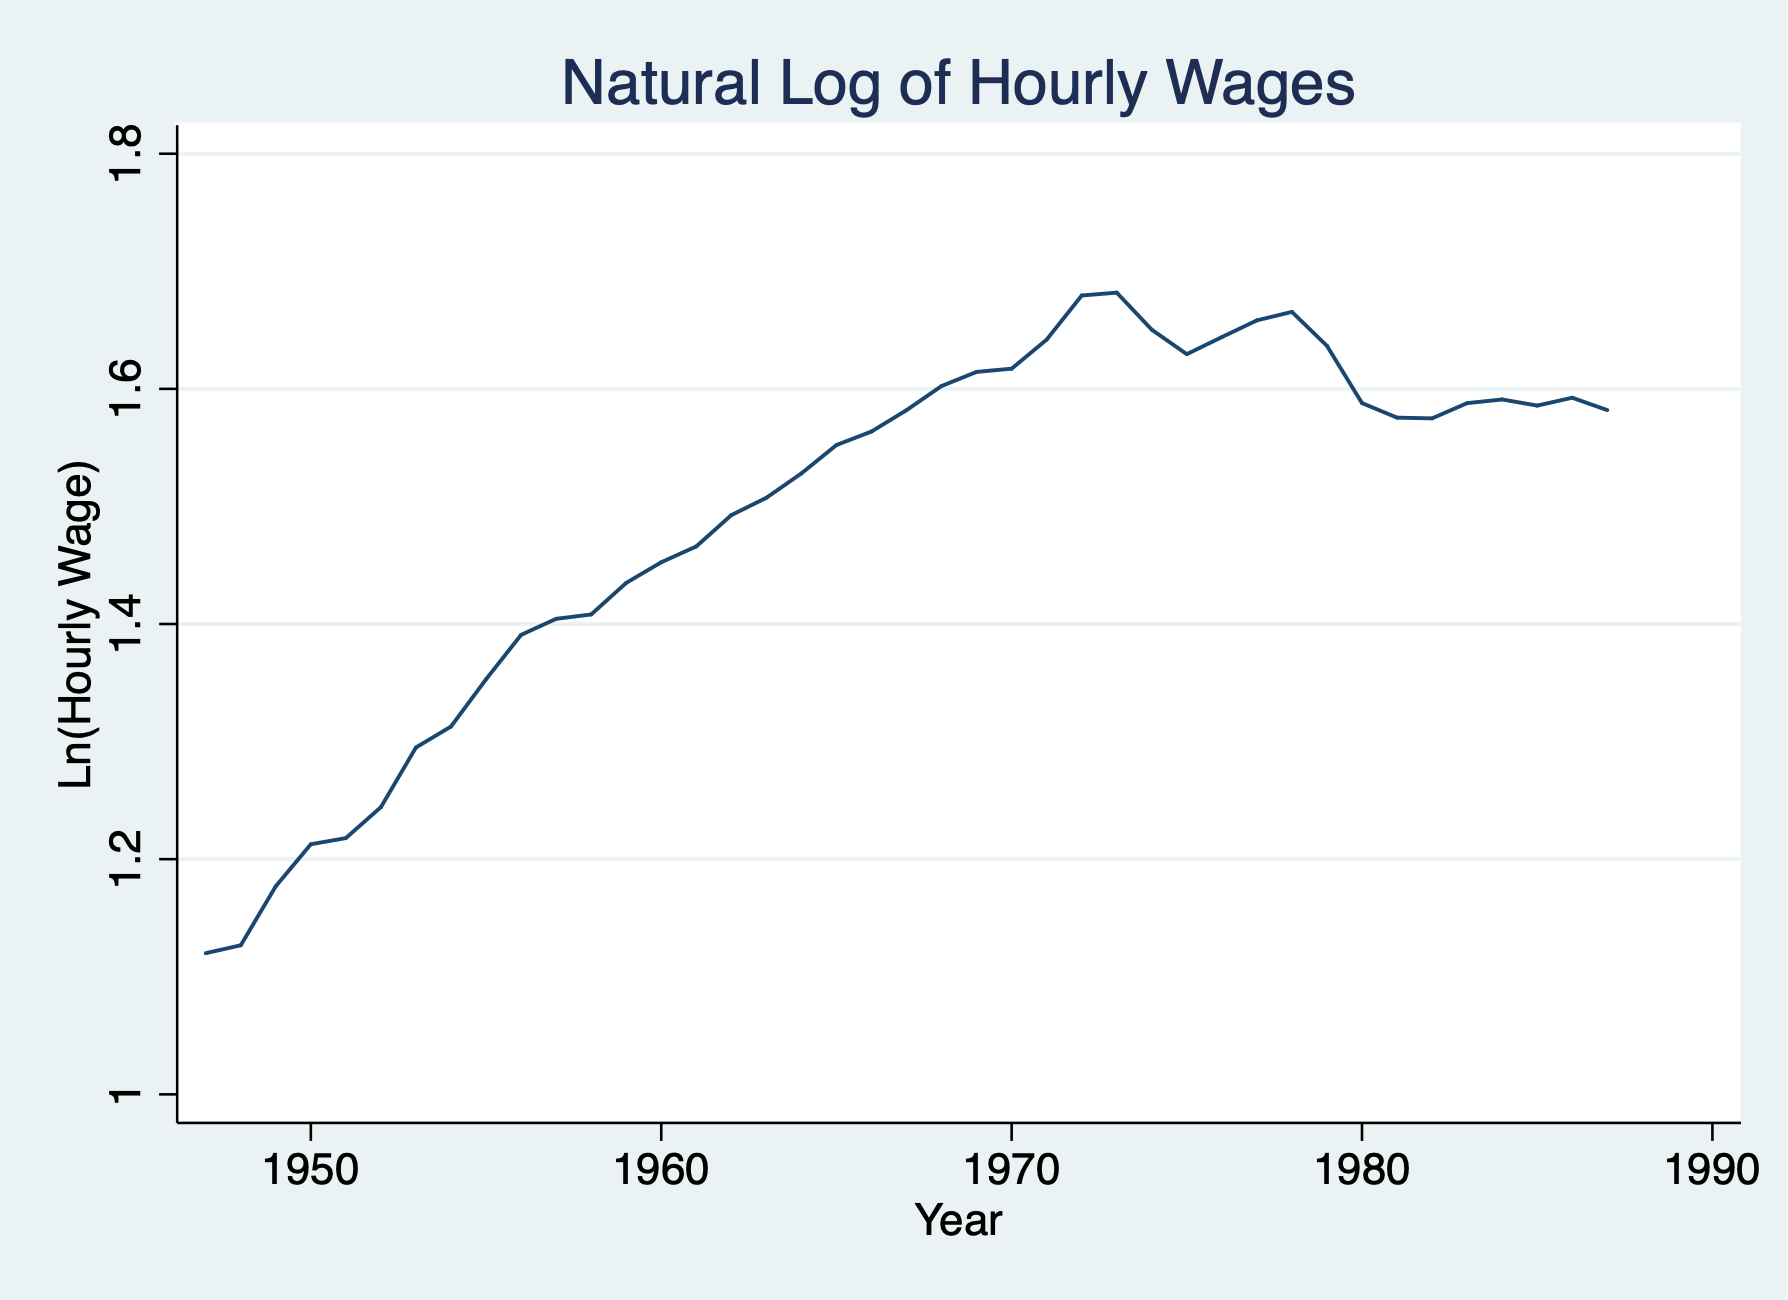
\includegraphics[keepaspectratio]{week_11_hrwage1.png}}
\caption{Natural Log of Hourly Wages}
\end{figure}

\begin{Shaded}
\begin{Highlighting}[]
    \KeywordTok{twoway} \KeywordTok{line} \KeywordTok{d}\NormalTok{.lhrwage }\FunctionTok{year}\NormalTok{, }\BaseNTok{title}\NormalTok{(}\StringTok{"First{-}Difference in Ln(Hourly Wages)"}\NormalTok{) }\BaseNTok{ytitle}\NormalTok{(}\StringTok{"Delta Ln(Hourly Wage)"}\NormalTok{) }\BaseNTok{xtitle}\NormalTok{(}\StringTok{"Year"}\NormalTok{)}
    \KeywordTok{graph} \KeywordTok{export} \StringTok{"/Users/Sam/Desktop/Econ 645/Stata/week\_11\_hrwage2.png"}\NormalTok{, }\KeywordTok{replace}
\end{Highlighting}
\end{Shaded}

\begin{figure}
\centering
\pandocbounded{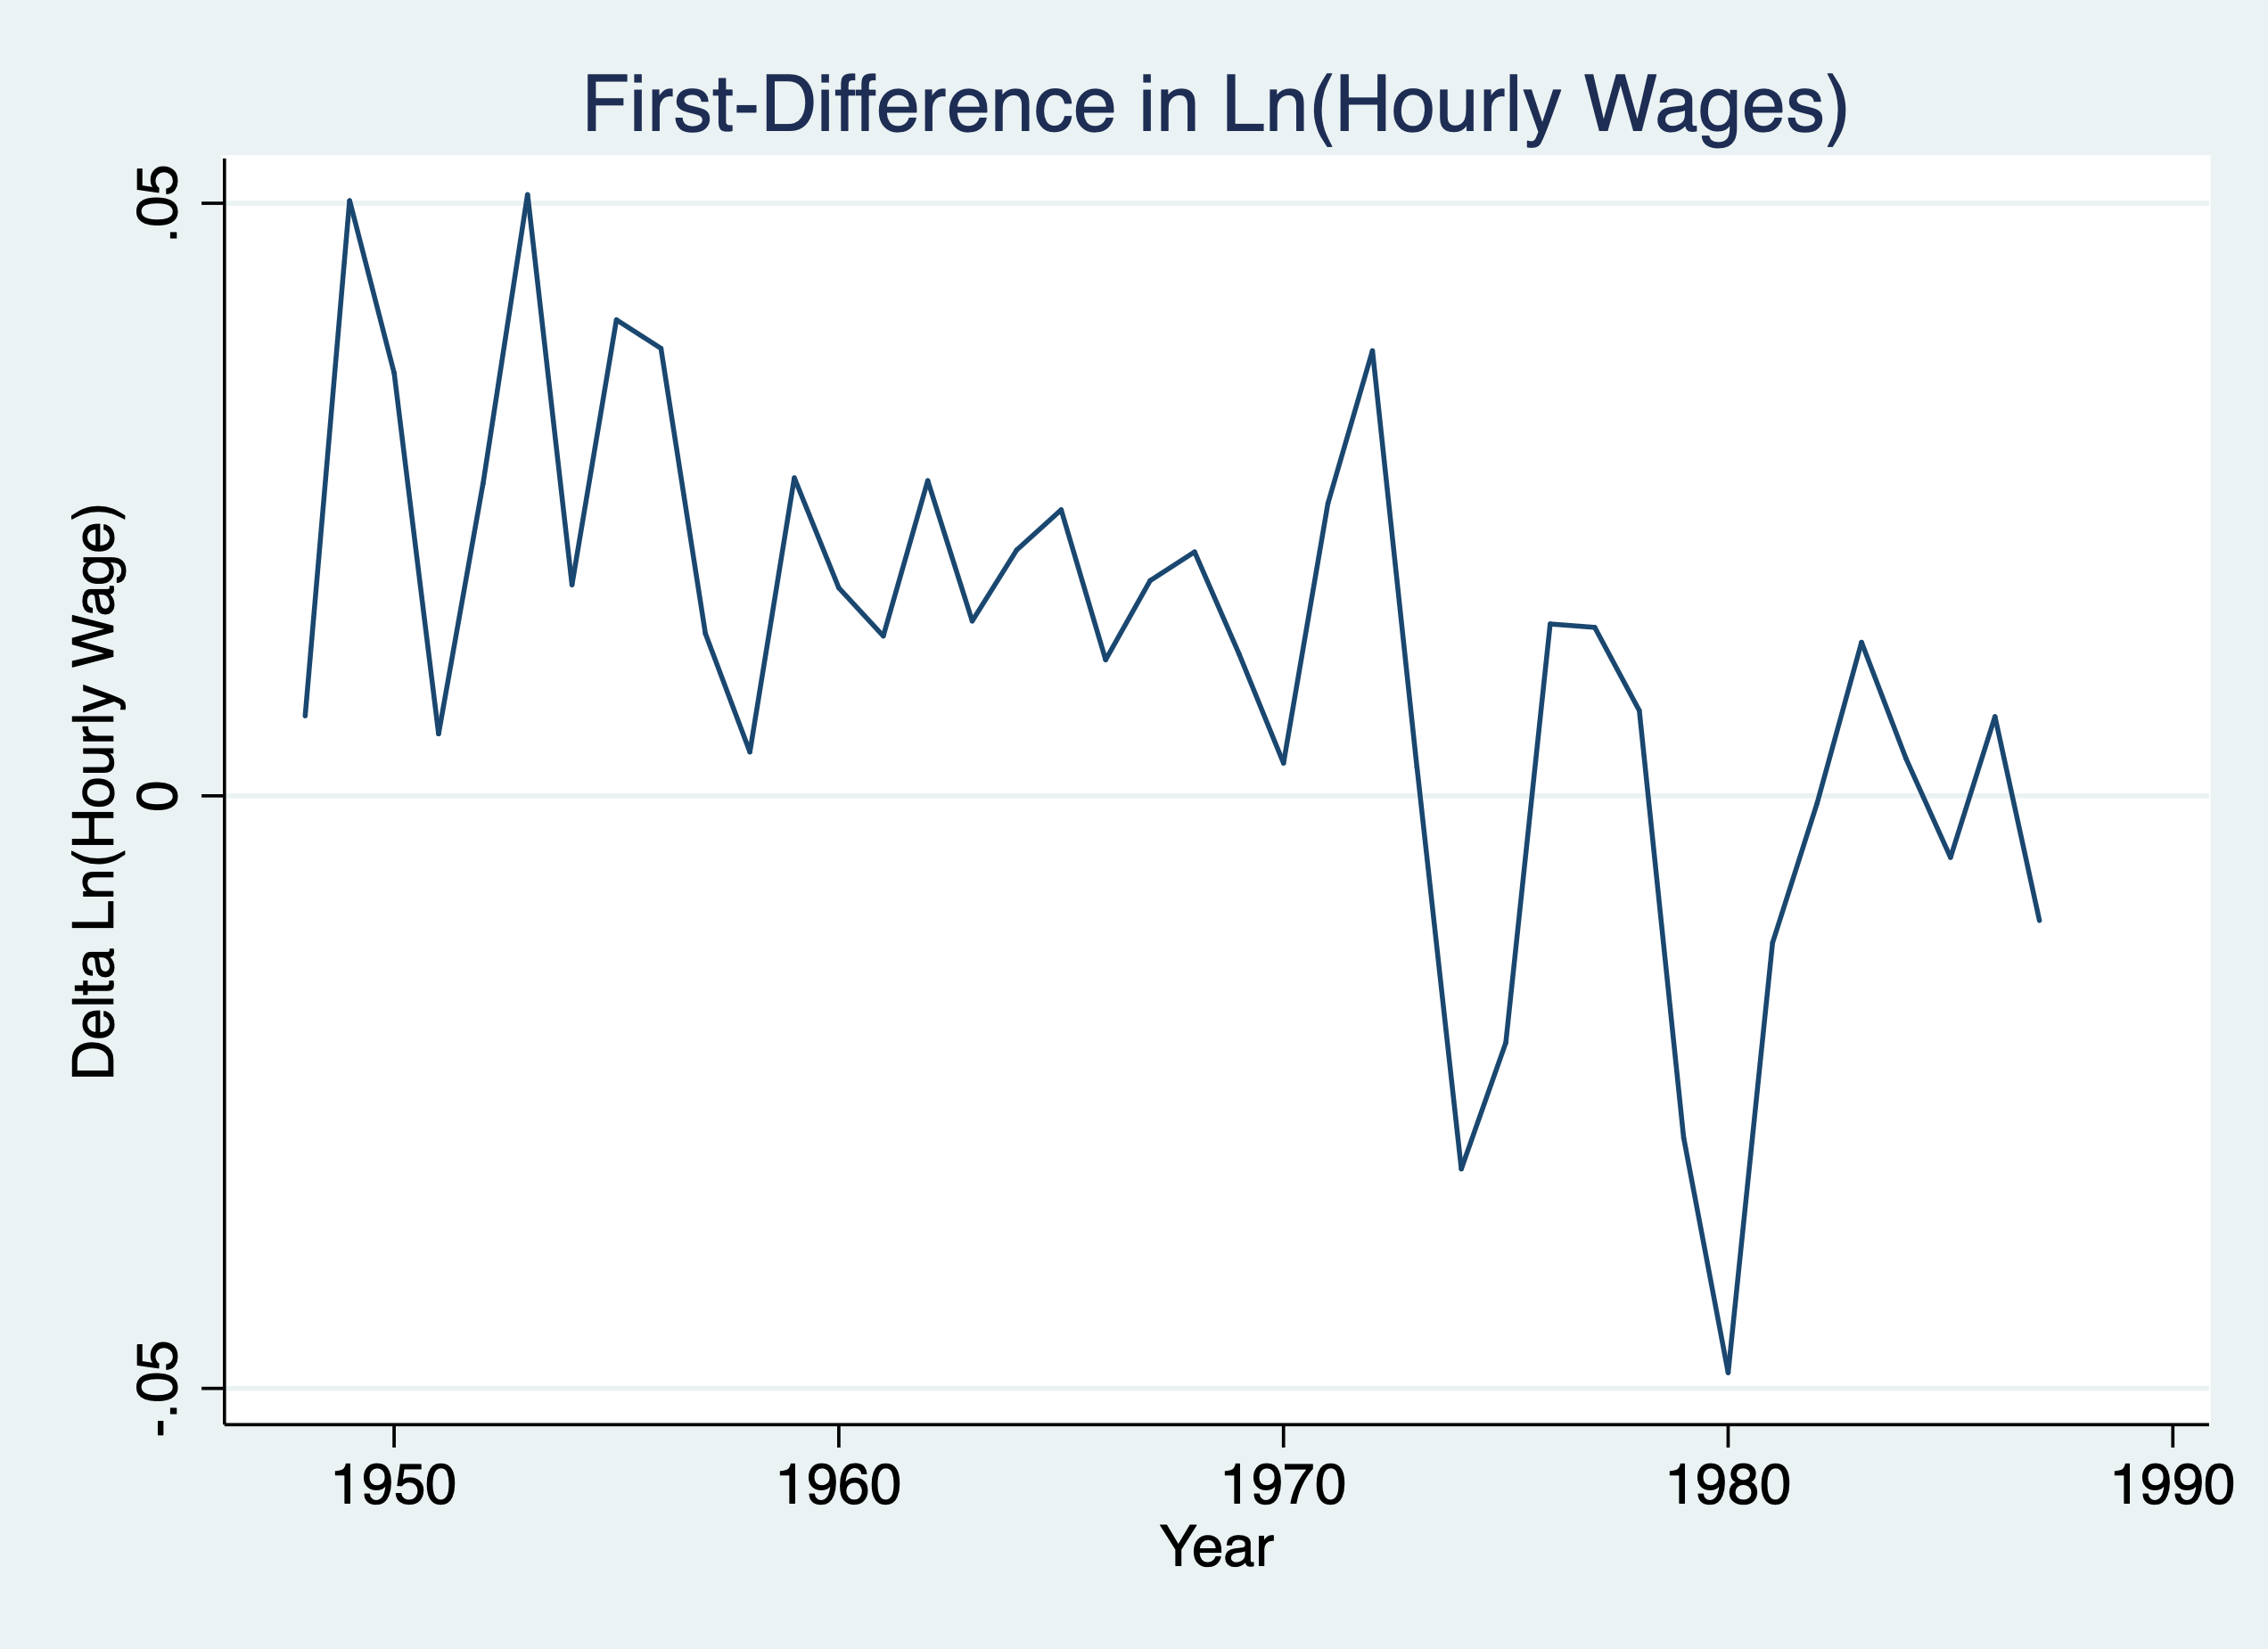
\includegraphics[keepaspectratio]{week_11_hrwage2.png}}
\caption{Difference in LN of Hourly Wage}
\end{figure}

We'll keep the trend based upon our prior graph

\begin{Shaded}
\begin{Highlighting}[]
\KeywordTok{reg} \KeywordTok{d}\NormalTok{.lhrwage }\KeywordTok{d}\NormalTok{.loutphr t}
\end{Highlighting}
\end{Shaded}

\begin{verbatim}
      Source |       SS           df       MS      Number of obs   =        40
-------------+----------------------------------   F(2, 37)        =     19.12
       Model |  .008727211         2  .004363605   Prob > F        =    0.0000
    Residual |  .008445792        37  .000228265   R-squared       =    0.5082
-------------+----------------------------------   Adj R-squared   =    0.4816
       Total |  .017173003        39  .000440333   Root MSE        =    .01511

------------------------------------------------------------------------------
   D.lhrwage |      Coef.   Std. Err.      t    P>|t|     [95% Conf. Interval]
-------------+----------------------------------------------------------------
     loutphr |
         D1. |   .5511404   .1733698     3.18   0.003     .1998598    .9024209
             |
           t |  -.0007637   .0002321    -3.29   0.002    -.0012339   -.0002935
       _cons |   .0176094   .0074784     2.35   0.024     .0024567    .0327622
------------------------------------------------------------------------------
\end{verbatim}

Our transformed model shows that a 1\% increase in output per hour is associated
with a .55\% increase in hourly wage.

\chapter{Dynamically Complete}\label{dynamically-complete}

\textbf{Lesson:} Is our model dynamically complete? Use theory/literature, but test, test, test.

Set Time Series

\begin{Shaded}
\begin{Highlighting}[]
\NormalTok{cd }\StringTok{"/Users/Sam/Desktop/Econ 645/Data/Wooldridge"}
\KeywordTok{use}\NormalTok{ fertil3.dta}
\KeywordTok{tsset} \FunctionTok{year}\NormalTok{, }\FunctionTok{yearly}
\end{Highlighting}
\end{Shaded}

\begin{verbatim}
/Users/Sam/Desktop/Econ 645/Data/Wooldridge

        time variable:  year, 1913 to 1984
                delta:  1 year
\end{verbatim}

We'll estimate a Finite Distributed Lag model for the first difference of
general fertility onto the first difference of personal exemptions.
If our model is dynamically complete, then no additional lags of gfr or pe
are needed.

Our First-difference model with one lag of pe

\begin{Shaded}
\begin{Highlighting}[]
\KeywordTok{reg} \KeywordTok{d}\NormalTok{.gfr }\KeywordTok{d}\NormalTok{.pe }\KeywordTok{d}\NormalTok{.pe\_1 }\KeywordTok{if} \FunctionTok{year}\NormalTok{ \textless{} 1985}
\end{Highlighting}
\end{Shaded}

\begin{verbatim}
      Source |       SS           df       MS      Number of obs   =        70
-------------+----------------------------------   F(2, 67)        =      1.20
       Model |  43.7985353         2  21.8992676   Prob > F        =    0.3063
    Residual |  1218.19557        67  18.1820235   R-squared       =    0.0347
-------------+----------------------------------   Adj R-squared   =    0.0059
       Total |  1261.99411        69  18.2897697   Root MSE        =     4.264

------------------------------------------------------------------------------
       D.gfr |      Coef.   Std. Err.      t    P>|t|     [95% Conf. Interval]
-------------+----------------------------------------------------------------
          pe |
         D1. |  -.0456497   .0294689    -1.55   0.126    -.1044699    .0131704
             |
        pe_1 |
         D1. |   .0134149   .0295326     0.45   0.651    -.0455324    .0723623
             |
       _cons |  -.8372962   .5117337    -1.64   0.106    -1.858721    .1841286
------------------------------------------------------------------------------
\end{verbatim}

Is this dynamically complete? Let's add a second lag of pe

\begin{Shaded}
\begin{Highlighting}[]
\KeywordTok{reg} \KeywordTok{d}\NormalTok{.gfr }\KeywordTok{d}\NormalTok{.pe }\KeywordTok{d}\NormalTok{.pe\_1 }\KeywordTok{d}\NormalTok{.pe\_2 }\KeywordTok{if} \FunctionTok{year}\NormalTok{ \textless{} 1985}
\end{Highlighting}
\end{Shaded}

\begin{verbatim}
      Source |       SS           df       MS      Number of obs   =        69
-------------+----------------------------------   F(3, 65)        =      6.56
       Model |  293.259859         3  97.7532864   Prob > F        =    0.0006
    Residual |  968.199959        65   14.895384   R-squared       =    0.2325
-------------+----------------------------------   Adj R-squared   =    0.1971
       Total |  1261.45982        68  18.5508797   Root MSE        =    3.8595

------------------------------------------------------------------------------
       D.gfr |      Coef.   Std. Err.      t    P>|t|     [95% Conf. Interval]
-------------+----------------------------------------------------------------
          pe |
         D1. |  -.0362021   .0267737    -1.35   0.181     -.089673    .0172687
             |
        pe_1 |
         D1. |  -.0139706   .0275539    -0.51   0.614    -.0689997    .0410584
             |
        pe_2 |
         D1. |   .1099896   .0268797     4.09   0.000     .0563071    .1636721
             |
       _cons |  -.9636787   .4677599    -2.06   0.043     -1.89786   -.0294976
------------------------------------------------------------------------------
\end{verbatim}

Add lag of d.gfr and see it wasn't dynamically complete

\begin{Shaded}
\begin{Highlighting}[]
\KeywordTok{reg} \KeywordTok{d}\NormalTok{.gfr }\KeywordTok{d}\NormalTok{.gfr\_1 }\KeywordTok{d}\NormalTok{.pe }\KeywordTok{d}\NormalTok{.pe\_1 }\KeywordTok{d}\NormalTok{.pe\_2 }\KeywordTok{if} \FunctionTok{year}\NormalTok{ \textless{} 1985}
\end{Highlighting}
\end{Shaded}

\begin{verbatim}
      Source |       SS           df       MS      Number of obs   =        69
-------------+----------------------------------   F(4, 64)        =      7.46
       Model |  401.286162         4   100.32154   Prob > F        =    0.0001
    Residual |  860.173657        64  13.4402134   R-squared       =    0.3181
-------------+----------------------------------   Adj R-squared   =    0.2755
       Total |  1261.45982        68  18.5508797   Root MSE        =    3.6661

------------------------------------------------------------------------------
       D.gfr |      Coef.   Std. Err.      t    P>|t|     [95% Conf. Interval]
-------------+----------------------------------------------------------------
       gfr_1 |
         D1. |   .3002422   .1059034     2.84   0.006     .0886758    .5118086
             |
          pe |
         D1. |  -.0454721   .0256417    -1.77   0.081    -.0966972     .005753
             |
        pe_1 |
         D1. |    .002064   .0267776     0.08   0.939    -.0514303    .0555584
             |
        pe_2 |
         D1. |   .1051346   .0255904     4.11   0.000      .054012    .1562572
             |
       _cons |  -.7021594   .4537988    -1.55   0.127    -1.608727    .2044079
------------------------------------------------------------------------------
\end{verbatim}

\chapter{Testing for Serial Correlation}\label{testing-for-serial-correlation}

\section{Example: Revisit Phillip's Curve}\label{example-revisit-phillips-curve}

\textbf{Lesson:} using our t-test, Durban Watson test, Breusch-Godfrey test, and Durban's alternative statistic to test for serial correlation

We'll use our t-test for serial correlation with strictly exogenous regressors
under the assumption that our regressors are exogenous.

Set Time Series

\begin{Shaded}
\begin{Highlighting}[]
\NormalTok{cd }\StringTok{"/Users/Sam/Desktop/Econ 645/Data/Wooldridge"}
\KeywordTok{use}\NormalTok{ phillips.dta, }\KeywordTok{clear}
\KeywordTok{tsset} \FunctionTok{year}\NormalTok{, }\FunctionTok{yearly}
\end{Highlighting}
\end{Shaded}

\begin{verbatim}
/Users/Sam/Desktop/Econ 645/Data/Wooldridge

        time variable:  year, 1948 to 2003
                delta:  1 year
\end{verbatim}

We estimated a static Phillips Curve and an augmented Phillips Curve last week.
We'll retest the models for serial correlation.

\subsection*{Static Model}\label{static-model}
\addcontentsline{toc}{subsection}{Static Model}

Test for serial correlation in Static Model
Noticeable serial correlation

\begin{Shaded}
\begin{Highlighting}[]
\NormalTok{*Static Model}
\KeywordTok{reg}\NormalTok{ inf unem }\KeywordTok{if} \FunctionTok{year}\NormalTok{ \textless{} 1997}

\NormalTok{*Heteroskedastiity Test: Breusch{-}Godfrey Test}
\KeywordTok{estat} \KeywordTok{bgodfrey}

\NormalTok{*Serial Correlation Test: Simple AR(1) }\KeywordTok{test}
\KeywordTok{predict}\NormalTok{ u, }\KeywordTok{resid}

\KeywordTok{reg}\NormalTok{ u }\OtherTok{l}\NormalTok{.u, noconst}
\end{Highlighting}
\end{Shaded}

\begin{verbatim}
      Source |       SS           df       MS      Number of obs   =        49
-------------+----------------------------------   F(1, 47)        =      2.62
       Model |  25.6369575         1  25.6369575   Prob > F        =    0.1125
    Residual |   460.61979        47  9.80042107   R-squared       =    0.0527
-------------+----------------------------------   Adj R-squared   =    0.0326
       Total |  486.256748        48  10.1303489   Root MSE        =    3.1306

------------------------------------------------------------------------------
         inf |      Coef.   Std. Err.      t    P>|t|     [95% Conf. Interval]
-------------+----------------------------------------------------------------
        unem |   .4676257   .2891262     1.62   0.112    -.1140213    1.049273
       _cons |    1.42361   1.719015     0.83   0.412    -2.034602    4.881822
------------------------------------------------------------------------------


Breusch-Godfrey LM test for autocorrelation
---------------------------------------------------------------------------
    lags(p)  |          chi2               df                 Prob > chi2
-------------+-------------------------------------------------------------
       1     |         18.472               1                   0.0000
---------------------------------------------------------------------------
                        H0: no serial correlation

      Source |       SS           df       MS      Number of obs   =        55
-------------+----------------------------------   F(1, 54)        =     29.61
       Model |  161.010846         1  161.010846   Prob > F        =    0.0000
    Residual |  293.652171        54  5.43800317   R-squared       =    0.3541
-------------+----------------------------------   Adj R-squared   =    0.3422
       Total |  454.663017        55  8.26660031   Root MSE        =     2.332

------------------------------------------------------------------------------
           u |      Coef.   Std. Err.      t    P>|t|     [95% Conf. Interval]
-------------+----------------------------------------------------------------
           u |
         L1. |   .5822453   .1070035     5.44   0.000     .3677161    .7967745
------------------------------------------------------------------------------
\end{verbatim}

\subsection*{First difference}\label{first-difference}
\addcontentsline{toc}{subsection}{First difference}

Test for serial correlation in Augmented
Serial correlation is removed with the first-difference in inflation

\begin{Shaded}
\begin{Highlighting}[]
\NormalTok{*First Difference Model}
\KeywordTok{reg} \KeywordTok{d}\NormalTok{.inf unem }\KeywordTok{if} \FunctionTok{year}\NormalTok{ \textless{} 1997}
\KeywordTok{predict}\NormalTok{ u2, }\KeywordTok{resid}
\NormalTok{*Breusch{-}Godfrey Test}
    \KeywordTok{estat} \KeywordTok{bgodfrey}
\end{Highlighting}
\end{Shaded}

\begin{verbatim}
      Source |       SS           df       MS      Number of obs   =        48
-------------+----------------------------------   F(1, 46)        =      5.56
       Model |  33.3829996         1  33.3829996   Prob > F        =    0.0227
    Residual |  276.305138        46  6.00663344   R-squared       =    0.1078
-------------+----------------------------------   Adj R-squared   =    0.0884
       Total |  309.688138        47  6.58910932   Root MSE        =    2.4508

------------------------------------------------------------------------------
       D.inf |      Coef.   Std. Err.      t    P>|t|     [95% Conf. Interval]
-------------+----------------------------------------------------------------
        unem |  -.5425869   .2301559    -2.36   0.023    -1.005867    -.079307
       _cons |   3.030581    1.37681     2.20   0.033      .259206    5.801955
------------------------------------------------------------------------------

(1 missing value generated)


Breusch-Godfrey LM test for autocorrelation
---------------------------------------------------------------------------
    lags(p)  |          chi2               df                 Prob > chi2
-------------+-------------------------------------------------------------
       1     |          0.062               1                   0.8039
---------------------------------------------------------------------------
                        H0: no serial correlation
\end{verbatim}

\subsection*{Test for Serial Correlation: Durban-Watson Test}\label{test-for-serial-correlation-durban-watson-test}
\addcontentsline{toc}{subsection}{Test for Serial Correlation: Durban-Watson Test}

\begin{Shaded}
\begin{Highlighting}[]
    \KeywordTok{estat}\NormalTok{ dwatson}
\end{Highlighting}
\end{Shaded}

\begin{verbatim}
Durbin-Watson d-statistic(  2,    48) =  1.769648
\end{verbatim}

\[ d_L = 1.503 \]
\[ d_U = 1.585 \]
\[ 1.769648 > 1.585 \]
We fail to reject the null hypothesis.

\subsection*{Test for Serial Correlation: AR(1) Test}\label{test-for-serial-correlation-ar1-test}
\addcontentsline{toc}{subsection}{Test for Serial Correlation: AR(1) Test}

\begin{Shaded}
\begin{Highlighting}[]
    \KeywordTok{reg}\NormalTok{ u2 }\OtherTok{l}\NormalTok{.u2, noconst}
\end{Highlighting}
\end{Shaded}

\begin{verbatim}
      Source |       SS           df       MS      Number of obs   =        54
-------------+----------------------------------   F(1, 53)        =      0.07
       Model |  .267251656         1  .267251656   Prob > F        =    0.7905
    Residual |  198.724905        53  3.74952651   R-squared       =    0.0013
-------------+----------------------------------   Adj R-squared   =   -0.0175
       Total |  198.992157        54  3.68503994   Root MSE        =    1.9364

------------------------------------------------------------------------------
          u2 |      Coef.   Std. Err.      t    P>|t|     [95% Conf. Interval]
-------------+----------------------------------------------------------------
          u2 |
         L1. |  -.0308131   .1154154    -0.27   0.791     -.262307    .2006808
------------------------------------------------------------------------------
\end{verbatim}

Test change in error terms for FD assumption on serial correlation so that
the differences in errors are not correlated.

\begin{Shaded}
\begin{Highlighting}[]
\KeywordTok{gen}\NormalTok{ u2\_1=}\OtherTok{l}\NormalTok{.u2}
\KeywordTok{reg} \KeywordTok{d}\NormalTok{.u2 }\KeywordTok{d}\NormalTok{.u2\_1, noconst}
\KeywordTok{drop}\NormalTok{ u2}
\end{Highlighting}
\end{Shaded}

\begin{verbatim}
(2 missing values generated)

      Source |       SS           df       MS      Number of obs   =        53
-------------+----------------------------------   F(1, 52)        =      2.01
       Model |  13.6239993         1  13.6239993   Prob > F        =    0.1623
    Residual |  352.532902        52  6.77947888   R-squared       =    0.0372
-------------+----------------------------------   Adj R-squared   =    0.0187
       Total |  366.156901        53  6.90862078   Root MSE        =    2.6037

------------------------------------------------------------------------------
        D.u2 |      Coef.   Std. Err.      t    P>|t|     [95% Conf. Interval]
-------------+----------------------------------------------------------------
        u2_1 |
         D1. |  -.1661051   .1171734    -1.42   0.162    -.4012307    .0690204
------------------------------------------------------------------------------
\end{verbatim}

We fail to reject the null hypothesis that there is no serial correlation in
the difference in error term.

\subsection*{FDL Model}\label{fdl-model}
\addcontentsline{toc}{subsection}{FDL Model}

Let's add a lag in inflation to change our static model into a FDL model.
We can also use the estat dwatson or dwstat

\begin{Shaded}
\begin{Highlighting}[]
\KeywordTok{reg}\NormalTok{ inf }\OtherTok{l}\NormalTok{.inf unem }\KeywordTok{if} \FunctionTok{year}\NormalTok{ \textless{} 1997}
\KeywordTok{estat}\NormalTok{ dwatson}
\NormalTok{*Or}
\KeywordTok{dwstat}
\end{Highlighting}
\end{Shaded}

\begin{verbatim}
      Source |       SS           df       MS      Number of obs   =        48
-------------+----------------------------------   F(2, 45)        =     19.72
       Model |  219.518187         2  109.759094   Prob > F        =    0.0000
    Residual |  250.471823        45  5.56604051   R-squared       =    0.4671
-------------+----------------------------------   Adj R-squared   =    0.4434
       Total |   469.99001        47  9.99978744   Root MSE        =    2.3592

------------------------------------------------------------------------------
         inf |      Coef.   Std. Err.      t    P>|t|     [95% Conf. Interval]
-------------+----------------------------------------------------------------
         inf |
         L1. |   .7278693   .1263167     5.76   0.000     .4734544    .9822841
             |
        unem |  -.2443814     .26124    -0.94   0.355    -.7705457    .2817829
       _cons |    2.43082   1.354276     1.79   0.079    -.2968325    5.158473
------------------------------------------------------------------------------


Durbin-Watson d-statistic(  3,    48) =  1.477467


Durbin-Watson d-statistic(  3,    48) =  1.477467
\end{verbatim}

First, let's find our critical values:
https://www3.nd.edu/\textasciitilde wevans1/econ30331/Durbin\_Watson\_tables.pdf.
\[ DW(3,48)=1.48 \] and \[ d_L \approx 1.4 \] and \[ d_U \approx 1.67 \]
so our DW test is inconclusive. We'll look at Durban-Watson and DW Tables again a bit later.

\section{Example: Revisit Puerto Rican Employment and Minimum Wage}\label{example-revisit-puerto-rican-employment-and-minimum-wage}

\textbf{Lesson:} We can use Durban's alternative statistic to test for serial correlation
if our regressors are not strictly exogenous.

Durban's alternative statistic

Set Time Series

\begin{Shaded}
\begin{Highlighting}[]
\NormalTok{cd }\StringTok{"/Users/Sam/Desktop/Econ 645/Data/Wooldridge"}
\KeywordTok{use}\NormalTok{ prminwge, }\KeywordTok{clear}
\KeywordTok{tsset} \FunctionTok{year}
\end{Highlighting}
\end{Shaded}

\begin{verbatim}
/Users/Sam/Desktop/Econ 645/Data/Wooldridge

        time variable:  year, 1950 to 1987
                delta:  1 unit
\end{verbatim}

We'll rerun our static model and regress the natural log of the employment-population
ratio onto the natural log of the importance of minimum wage, the natural log
of Puerto Rican Gross National Product, the natural log of US GNP, and a time trend.

\subsection*{Durbin-Watson Test}\label{durbin-watson-test}
\addcontentsline{toc}{subsection}{Durbin-Watson Test}

\begin{Shaded}
\begin{Highlighting}[]
\KeywordTok{reg}\NormalTok{ lprepop lmincov lprgnp lusgnp t }\KeywordTok{if} \FunctionTok{year}\NormalTok{ \textless{} 1988}
\KeywordTok{predict}\NormalTok{ u, }\KeywordTok{resid}
\end{Highlighting}
\end{Shaded}

\begin{verbatim}
      Source |       SS           df       MS      Number of obs   =        38
-------------+----------------------------------   F(4, 33)        =     66.23
       Model |  .284430187         4  .071107547   Prob > F        =    0.0000
    Residual |  .035428331        33  .001073586   R-squared       =    0.8892
-------------+----------------------------------   Adj R-squared   =    0.8758
       Total |  .319858518        37  .008644825   Root MSE        =    .03277

------------------------------------------------------------------------------
     lprepop |      Coef.   Std. Err.      t    P>|t|     [95% Conf. Interval]
-------------+----------------------------------------------------------------
     lmincov |  -.2122612   .0401524    -5.29   0.000    -.2939518   -.1305706
      lprgnp |   .2852386   .0804922     3.54   0.001      .121476    .4490012
      lusgnp |   .4860463   .2219829     2.19   0.036     .0344188    .9376739
           t |  -.0266633   .0046267    -5.76   0.000    -.0360765   -.0172502
       _cons |  -6.663432   1.257831    -5.30   0.000    -9.222508   -4.104356
------------------------------------------------------------------------------
\end{verbatim}

\subsection*{Durbin's Alternative Statistics}\label{durbins-alternative-statistics}
\addcontentsline{toc}{subsection}{Durbin's Alternative Statistics}

Test Serial Correlation with Durbin's alternative statistic, which is valid when
we don't have strictly exogenous regressors.

\begin{Shaded}
\begin{Highlighting}[]
\KeywordTok{reg}\NormalTok{ u }\OtherTok{l}\NormalTok{.u lmincov lprgnp lusgnp t, noconst }
\end{Highlighting}
\end{Shaded}

\begin{verbatim}
      Source |       SS           df       MS      Number of obs   =        37
-------------+----------------------------------   F(5, 32)        =      1.92
       Model |  .007182064         5  .001436413   Prob > F        =    0.1191
    Residual |  .023990478        32  .000749702   R-squared       =    0.2304
-------------+----------------------------------   Adj R-squared   =    0.1101
       Total |  .031172542        37  .000842501   Root MSE        =    .02738

------------------------------------------------------------------------------
           u |      Coef.   Std. Err.      t    P>|t|     [95% Conf. Interval]
-------------+----------------------------------------------------------------
           u |
         L1. |   .4757945   .1653074     2.88   0.007     .1390742    .8125147
             |
     lmincov |    .041425   .0346345     1.20   0.240    -.0291232    .1119732
      lprgnp |  -.0522061   .0615544    -0.85   0.403    -.1775883    .0731762
      lusgnp |   .0606233   .0644769     0.94   0.354     -.070712    .1919585
           t |  -.0005264   .0015194    -0.35   0.731    -.0036213    .0025685
------------------------------------------------------------------------------
\end{verbatim}

We can see that we reject the null hypothesis, since our \(\hat{rho} = 0.48\) and
statistically significant.

\section{Test AR(3) serial correlation}\label{test-ar3-serial-correlation}

\textbf{Lesson:} We can test for serial correlation among prior periods beside AR(1).

Set Time Series

\begin{Shaded}
\begin{Highlighting}[]
\NormalTok{cd }\StringTok{"/Users/Sam/Desktop/Econ 645/Data/Wooldridge"}
\KeywordTok{use}\NormalTok{ barium.dta, }\KeywordTok{clear}
\KeywordTok{tsset}\NormalTok{ t, }\FunctionTok{monthly}
\end{Highlighting}
\end{Shaded}

\begin{verbatim}
/Users/Sam/Desktop/Econ 645/Data/Wooldridge

        time variable:  t, 1960m2 to 1970m12
                delta:  1 month
\end{verbatim}

We'll look at our barium chloride model again to see if ITC complaints affect
behavior of foreign exporters. We may have higher order of serial correlation
since we are using monthly data.

\begin{Shaded}
\begin{Highlighting}[]
\KeywordTok{reg}\NormalTok{ lchnimp lchempi lgas lrtwex befile6 affile6 afdec6}
\KeywordTok{predict}\NormalTok{ u, }\KeywordTok{resid}
\end{Highlighting}
\end{Shaded}

\begin{verbatim}
      Source |       SS           df       MS      Number of obs   =       131
-------------+----------------------------------   F(6, 124)       =      9.06
       Model |  19.4051607         6  3.23419346   Prob > F        =    0.0000
    Residual |  44.2470875       124  .356831351   R-squared       =    0.3049
-------------+----------------------------------   Adj R-squared   =    0.2712
       Total |  63.6522483       130  .489632679   Root MSE        =    .59735

------------------------------------------------------------------------------
     lchnimp |      Coef.   Std. Err.      t    P>|t|     [95% Conf. Interval]
-------------+----------------------------------------------------------------
     lchempi |   3.117193   .4792021     6.50   0.000     2.168718    4.065668
        lgas |   .1963504   .9066172     0.22   0.829    -1.598099      1.9908
      lrtwex |   .9830183   .4001537     2.46   0.015     .1910022    1.775034
     befile6 |   .0595739   .2609699     0.23   0.820    -.4569585    .5761064
     affile6 |  -.0324064   .2642973    -0.12   0.903    -.5555249     .490712
      afdec6 |   -.565245   .2858352    -1.98   0.050    -1.130993    .0005028
       _cons |    -17.803   21.04537    -0.85   0.399    -59.45769    23.85169
------------------------------------------------------------------------------
\end{verbatim}

Test for \(H_{0}: p1=p2=p3=0\) jointly with an F-test.

\begin{Shaded}
\begin{Highlighting}[]
\KeywordTok{reg}\NormalTok{ u }\OtherTok{l}\NormalTok{.u l2.u l3.u lchempi lgas lrtwex befile6 affile6 afdec6, noconst}
\KeywordTok{test} \OtherTok{l}\NormalTok{.u l2.u l3.u}
\end{Highlighting}
\end{Shaded}

\begin{verbatim}
      Source |       SS           df       MS      Number of obs   =       128
-------------+----------------------------------   F(9, 119)       =      1.67
       Model |   4.8836741         9  .542630456   Prob > F        =    0.1024
    Residual |  38.5511192       119  .323958985   R-squared       =    0.1124
-------------+----------------------------------   Adj R-squared   =    0.0453
       Total |  43.4347933       128  .339334323   Root MSE        =    .56917

------------------------------------------------------------------------------
           u |      Coef.   Std. Err.      t    P>|t|     [95% Conf. Interval]
-------------+----------------------------------------------------------------
           u |
         L1. |    .215573   .0910635     2.37   0.020     .0352581    .3958878
         L2. |   .1296804   .0917465     1.41   0.160    -.0519868    .3113477
         L3. |   .1209405   .0906816     1.33   0.185    -.0586181    .3004992
             |
     lchempi |   -.105758   .4679356    -0.23   0.822    -1.032317    .8208012
        lgas |   .0125667   .1187882     0.11   0.916    -.2226459    .2477792
      lrtwex |   .0518992   .3452261     0.15   0.881     -.631683    .7354815
     befile6 |  -.0730016    .249775    -0.29   0.771     -.567581    .4215779
     affile6 |   -.122359   .2541453    -0.48   0.631    -.6255919     .380874
      afdec6 |  -.0694522   .2737453    -0.25   0.800    -.6114953    .4725909
------------------------------------------------------------------------------


 ( 1)  L.u = 0
 ( 2)  L2.u = 0
 ( 3)  L3.u = 0

       F(  3,   119) =    4.98
            Prob > F =    0.0027
\end{verbatim}

Our reject the null hypothesis that all of the lags are equal to zero using an F-test.

However, when we test our last two lags, they are jointly insignificant.

\begin{Shaded}
\begin{Highlighting}[]
\KeywordTok{test}\NormalTok{ l2.u l3.u}
\KeywordTok{drop}\NormalTok{ u}
\end{Highlighting}
\end{Shaded}

\begin{verbatim}
 ( 1)  L2.u = 0
 ( 2)  L3.u = 0

       F(  2,   119) =    2.42
            Prob > F =    0.0930
\end{verbatim}

We have evidence of at least serial correlation to the order of one.

\chapter{Correct for Serial Correlation}\label{correct-for-serial-correlation}

\section{Prais-Winsten Estimation in the Event Study}\label{prais-winsten-estimation-in-the-event-study}

\textbf{Lesson:} We'll account for serial correlation with a FGLS Prais-Winsten model.

Set Time Series

\begin{Shaded}
\begin{Highlighting}[]
\NormalTok{cd }\StringTok{"/Users/Sam/Desktop/Econ 645/Data/Wooldridge"}
\KeywordTok{use}\NormalTok{ barium.dta, }\KeywordTok{clear}
\KeywordTok{tsset}\NormalTok{ t, }\FunctionTok{monthly}
\end{Highlighting}
\end{Shaded}

\begin{verbatim}
/Users/Sam/Desktop/Econ 645/Data/Wooldridge

        time variable:  t, 1960m2 to 1970m12
                delta:  1 month
\end{verbatim}

\subsection*{OLS}\label{ols}
\addcontentsline{toc}{subsection}{OLS}

\begin{Shaded}
\begin{Highlighting}[]
\KeywordTok{est} \KeywordTok{clear}
\NormalTok{eststo OLS: }\KeywordTok{reg}\NormalTok{ lchnimp lchempi lgas lrtwex befile6 affile6 afdec6}
\KeywordTok{estat} \KeywordTok{dwstat}
\end{Highlighting}
\end{Shaded}

\begin{verbatim}
      Source |       SS           df       MS      Number of obs   =       131
-------------+----------------------------------   F(6, 124)       =      9.06
       Model |  19.4051607         6  3.23419346   Prob > F        =    0.0000
    Residual |  44.2470875       124  .356831351   R-squared       =    0.3049
-------------+----------------------------------   Adj R-squared   =    0.2712
       Total |  63.6522483       130  .489632679   Root MSE        =    .59735

------------------------------------------------------------------------------
     lchnimp |      Coef.   Std. Err.      t    P>|t|     [95% Conf. Interval]
-------------+----------------------------------------------------------------
     lchempi |   3.117193   .4792021     6.50   0.000     2.168718    4.065668
        lgas |   .1963504   .9066172     0.22   0.829    -1.598099      1.9908
      lrtwex |   .9830183   .4001537     2.46   0.015     .1910022    1.775034
     befile6 |   .0595739   .2609699     0.23   0.820    -.4569585    .5761064
     affile6 |  -.0324064   .2642973    -0.12   0.903    -.5555249     .490712
      afdec6 |   -.565245   .2858352    -1.98   0.050    -1.130993    .0005028
       _cons |    -17.803   21.04537    -0.85   0.399    -59.45769    23.85169
------------------------------------------------------------------------------


Durbin-Watson d-statistic(  7,   131) =  1.458414
\end{verbatim}

\subsection*{Prais-Winsten}\label{prais-winsten}
\addcontentsline{toc}{subsection}{Prais-Winsten}

\begin{Shaded}
\begin{Highlighting}[]
\NormalTok{eststo Prais: }\KeywordTok{prais}\NormalTok{ lchnimp lchempi lgas lrtwex befile6 affile6 afdec6}
\end{Highlighting}
\end{Shaded}

\begin{verbatim}
Iteration 0:  rho = 0.0000
Iteration 1:  rho = 0.2708
Iteration 2:  rho = 0.2910
Iteration 3:  rho = 0.2930
Iteration 4:  rho = 0.2932
Iteration 5:  rho = 0.2932
Iteration 6:  rho = 0.2932
Iteration 7:  rho = 0.2932

Prais-Winsten AR(1) regression -- iterated estimates

      Source |       SS           df       MS      Number of obs   =       131
-------------+----------------------------------   F(6, 124)       =      5.24
       Model |  10.3252323         6  1.72087205   Prob > F        =    0.0001
    Residual |  40.7593886       124  .328704747   R-squared       =    0.2021
-------------+----------------------------------   Adj R-squared   =    0.1635
       Total |  51.0846209       130  .392958622   Root MSE        =    .57333

------------------------------------------------------------------------------
     lchnimp |      Coef.   Std. Err.      t    P>|t|     [95% Conf. Interval]
-------------+----------------------------------------------------------------
     lchempi |   2.940949   .6328402     4.65   0.000     1.688381    4.193517
        lgas |    1.04638   .9773356     1.07   0.286    -.8880406    2.980801
      lrtwex |   1.132791   .5066578     2.24   0.027     .1299738    2.135609
     befile6 |  -.0164787   .3193802    -0.05   0.959    -.6486216    .6156641
     affile6 |  -.0331563   .3218101    -0.10   0.918    -.6701086     .603796
      afdec6 |  -.5768122   .3419865    -1.69   0.094    -1.253699    .1000748
       _cons |   -37.0777    22.7783    -1.63   0.106    -82.16235    8.006941
-------------+----------------------------------------------------------------
         rho |    .293217
------------------------------------------------------------------------------
Durbin-Watson statistic (original)    1.458414
Durbin-Watson statistic (transformed) 2.087181
\end{verbatim}

First, let's find our critical values:
https://www3.nd.edu/\textasciitilde wevans1/econ30331/Durbin\_Watson\_tables.pdf.
For the OLS Estimator
\[ DW(6,131) = 1.458414 \]
For the Prasi-Winsten Estimator
\[ DW(6,131) = 2.087181 \]
and \[ d_L \approx 1.60 \] and \[ d_U \approx 1.81 \]
We reject the null hypothesis for the OLS estimator, but we fail to reject
the null hypothesis for the Prais-Winsten Estimator.

Our beta-hats in Prais-Winsten Estimator are similar to our OLS estimates, but our PW
standard errors account for the serial correlation. Our OLS standard errors
usually understate the actual sampling variation in the OLS estimators and
should be treated with suspicion.

\begin{Shaded}
\begin{Highlighting}[]
\NormalTok{    esttab, mtitle se stat(}\KeywordTok{N}\NormalTok{ rho)}
\end{Highlighting}
\end{Shaded}

\begin{verbatim}
                      (1)             (2)   
                      OLS           Prais   
--------------------------------------------
lchempi             3.117***        2.941***
                  (0.479)         (0.633)   

lgas                0.196           1.046   
                  (0.907)         (0.977)   

lrtwex              0.983*          1.133*  
                  (0.400)         (0.507)   

befile6            0.0596         -0.0165   
                  (0.261)         (0.319)   

affile6           -0.0324         -0.0332   
                  (0.264)         (0.322)   

afdec6             -0.565          -0.577   
                  (0.286)         (0.342)   

_cons              -17.80          -37.08   
                  (21.05)         (22.78)   
--------------------------------------------
N                     131             131   
rho                                 0.293   
--------------------------------------------
Standard errors in parentheses
* p<0.05, ** p<0.01, *** p<0.001
\end{verbatim}

\section{Inflation and Prais}\label{inflation-and-prais}

\textbf{Lesson:} our PW estimator might not be unbiased or consistent if our assumptions fail.

We'll show another example comparing OLS and Prais-Winsten estimators. We'll
look at the static Phillips curve, which we know has serial correlation.

Set the Time Series

\begin{Shaded}
\begin{Highlighting}[]
\NormalTok{cd }\StringTok{"/Users/Sam/Desktop/Econ 645/Data/Wooldridge"}
\KeywordTok{use}\NormalTok{ phillips.dta, }\KeywordTok{clear}
\KeywordTok{tsset} \FunctionTok{year}
\KeywordTok{est} \KeywordTok{clear}
\end{Highlighting}
\end{Shaded}

\begin{verbatim}
/Users/Sam/Desktop/Econ 645/Data/Wooldridge

        time variable:  year, 1948 to 2003
                delta:  1 unit
\end{verbatim}

\subsection*{OLS}\label{ols-1}
\addcontentsline{toc}{subsection}{OLS}

\begin{Shaded}
\begin{Highlighting}[]
\KeywordTok{quietly}\NormalTok{ eststo OLS: }\KeywordTok{reg}\NormalTok{ inf unem }\KeywordTok{if} \FunctionTok{year}\NormalTok{ \textless{} 1997}
\end{Highlighting}
\end{Shaded}

\subsection*{Prais-Winsten}\label{prais-winsten-1}
\addcontentsline{toc}{subsection}{Prais-Winsten}

\begin{Shaded}
\begin{Highlighting}[]
\KeywordTok{quietly}\NormalTok{ eststo PW: }\KeywordTok{prais}\NormalTok{ inf unem }\KeywordTok{if} \FunctionTok{year}\NormalTok{ \textless{} 1997}
\end{Highlighting}
\end{Shaded}

\subsection*{Prais-Winsten with Cochrane-Orcutt Transformation}\label{prais-winsten-with-cochrane-orcutt-transformation}
\addcontentsline{toc}{subsection}{Prais-Winsten with Cochrane-Orcutt Transformation}

\begin{Shaded}
\begin{Highlighting}[]
\KeywordTok{quietly}\NormalTok{ eststo PW\_CO: }\KeywordTok{prais}\NormalTok{ inf unem }\KeywordTok{if} \FunctionTok{year}\NormalTok{ \textless{} 1997, }\KeywordTok{corc}
\end{Highlighting}
\end{Shaded}

\subsection*{First Difference}\label{first-difference-1}
\addcontentsline{toc}{subsection}{First Difference}

\begin{Shaded}
\begin{Highlighting}[]
\KeywordTok{quietly}\NormalTok{ eststo FD: }\KeywordTok{reg} \KeywordTok{d}\NormalTok{.inf }\KeywordTok{d}\NormalTok{.unem }\KeywordTok{if} \FunctionTok{year}\NormalTok{ \textless{} 1997}
\end{Highlighting}
\end{Shaded}

\subsection*{Compare}\label{compare}
\addcontentsline{toc}{subsection}{Compare}

\begin{Shaded}
\begin{Highlighting}[]
\NormalTok{    esttab, mtitle se stat(}\KeywordTok{N}\NormalTok{ rho)}
\end{Highlighting}
\end{Shaded}

\begin{verbatim}
                      (1)             (2)             (3)             (4)   
                      OLS              PW           PW_CO              FD   
----------------------------------------------------------------------------
unem                0.468          -0.716*         -0.665*                  
                  (0.289)         (0.313)         (0.320)                   

D.unem                                                             -0.842*  
                                                                  (0.314)   

_cons               1.424           8.296***        7.583**       -0.0782   
                  (1.719)         (2.231)         (2.381)         (0.348)   
----------------------------------------------------------------------------
N                      49              49              48              48   
rho                                 0.781           0.774                   
----------------------------------------------------------------------------
Standard errors in parentheses
* p<0.05, ** p<0.01, *** p<0.001
\end{verbatim}

The OLS and PW estimators might give very different estimators if our
assumptions of strict exogeneity and the a \(Cov(x_(t+1)+x_(t-1),u_t)=0\)
fail. If that is the case then using OLS with a first-difference might be
a better method.

We can see that the difference is quite notable. With our OLS estimators, the
tradeoff between inflation and employment is non-existent, but with the PW
estimator our estimate of beta 1 is closer to our first-difference estimate
of beta 1.

It is possible that there is no relationship with the static model, but
the change in inflation and the change in unemployment are negatively related.

\section{Differencing and Serial Correlation}\label{differencing-and-serial-correlation}

\subsection{Inflation and Deficits on Interest Rates}\label{inflation-and-deficits-on-interest-rates}

\textbf{Lesson:} First-differencing is a potential method to eliminate serial correlation.

Set the Time Series

\begin{Shaded}
\begin{Highlighting}[]
\NormalTok{cd }\StringTok{"/Users/Sam/Desktop/Econ 645/Data/Wooldridge"}
\KeywordTok{use}\NormalTok{ intdef.dta, }\KeywordTok{clear}
\KeywordTok{tsset} \FunctionTok{year}
\end{Highlighting}
\end{Shaded}

\begin{verbatim}
/Users/Sam/Desktop/Econ 645/Data/Wooldridge

        time variable:  year, 1948 to 2003
                delta:  1 unit
\end{verbatim}

We'll look at the relationship between interest rates from the 3-month T-bill rate (i3)
and inflation rate (inf) and deficits as a percentage of GDP.

\subsection*{Static Model}\label{static-model-1}
\addcontentsline{toc}{subsection}{Static Model}

Calculate a static model and test for serial correlation

\begin{Shaded}
\begin{Highlighting}[]
\KeywordTok{reg}\NormalTok{ i3 inf def }\KeywordTok{if} \FunctionTok{year}\NormalTok{ \textless{} 2004}
\KeywordTok{estat} \KeywordTok{dwstat}
\end{Highlighting}
\end{Shaded}

\begin{verbatim}
      Source |       SS           df       MS      Number of obs   =        56
-------------+----------------------------------   F(2, 53)        =     40.09
       Model |  272.420338         2  136.210169   Prob > F        =    0.0000
    Residual |  180.054275        53  3.39725047   R-squared       =    0.6021
-------------+----------------------------------   Adj R-squared   =    0.5871
       Total |  452.474612        55  8.22681113   Root MSE        =    1.8432

------------------------------------------------------------------------------
          i3 |      Coef.   Std. Err.      t    P>|t|     [95% Conf. Interval]
-------------+----------------------------------------------------------------
         inf |   .6058659   .0821348     7.38   0.000     .4411243    .7706074
         def |   .5130579   .1183841     4.33   0.000     .2756095    .7505062
       _cons |   1.733266    .431967     4.01   0.000     .8668497    2.599682
------------------------------------------------------------------------------


Durbin-Watson d-statistic(  3,    56) =  .7161527
\end{verbatim}

Critical values \(d(3,56)=.716\), at the 5\% level \(dL = 1.452, dU=1.681\)
\(dwstat < dL\) so we reject the null hypothesis

\begin{Shaded}
\begin{Highlighting}[]
\KeywordTok{predict}\NormalTok{ u, }\KeywordTok{resid}
\KeywordTok{reg}\NormalTok{ u }\OtherTok{l}\NormalTok{.u, noconst}
\KeywordTok{drop}\NormalTok{ u}
\end{Highlighting}
\end{Shaded}

\begin{verbatim}
      Source |       SS           df       MS      Number of obs   =        55
-------------+----------------------------------   F(1, 54)        =     32.83
       Model |  64.1034163         1  64.1034163   Prob > F        =    0.0000
    Residual |  105.448636        54  1.95275252   R-squared       =    0.3781
-------------+----------------------------------   Adj R-squared   =    0.3666
       Total |  169.552053        55  3.08276459   Root MSE        =    1.3974

------------------------------------------------------------------------------
           u |      Coef.   Std. Err.      t    P>|t|     [95% Conf. Interval]
-------------+----------------------------------------------------------------
           u |
         L1. |   .6228816   .1087148     5.73   0.000     .4049216    .8408415
------------------------------------------------------------------------------
\end{verbatim}

We find that we have notable serial correlation in the error term that is statistically
significant. We'll run a first-difference model next.

\subsection*{First differencing}\label{first-differencing}
\addcontentsline{toc}{subsection}{First differencing}

Run a first-difference and test for serial correlation

\begin{Shaded}
\begin{Highlighting}[]
\KeywordTok{reg} \KeywordTok{d}\NormalTok{.i3 }\KeywordTok{d}\NormalTok{.inf }\KeywordTok{d}\NormalTok{.def }\KeywordTok{if} \FunctionTok{year}\NormalTok{ \textless{} 2004}
\KeywordTok{dwstat}
\end{Highlighting}
\end{Shaded}

\begin{verbatim}
      Source |       SS           df       MS      Number of obs   =        55
-------------+----------------------------------   F(2, 52)        =      5.57
       Model |  17.8058164         2  8.90290822   Prob > F        =    0.0065
    Residual |  83.1753707        52  1.59952636   R-squared       =    0.1763
-------------+----------------------------------   Adj R-squared   =    0.1446
       Total |  100.981187        54  1.87002198   Root MSE        =    1.2647

------------------------------------------------------------------------------
        D.i3 |      Coef.   Std. Err.      t    P>|t|     [95% Conf. Interval]
-------------+----------------------------------------------------------------
         inf |
         D1. |   .1494892   .0921555     1.62   0.111    -.0354343    .3344127
             |
         def |
         D1. |  -.1813151   .1476825    -1.23   0.225    -.4776618    .1150315
             |
       _cons |   .0417738   .1713874     0.24   0.808    -.3021401    .3856877
------------------------------------------------------------------------------


Durbin-Watson d-statistic(  3,    55) =  1.796365
\end{verbatim}

Critical values \(d(3,56)=1.796\), at the 5\% level \(dL = 1.452, dU=1.681\)
\(dwstat > dU\) so we fail to reject the null hypothesis

\begin{Shaded}
\begin{Highlighting}[]
\KeywordTok{predict}\NormalTok{ u, }\KeywordTok{resid}
\KeywordTok{reg}\NormalTok{ u }\OtherTok{l}\NormalTok{.u, noconst}
\end{Highlighting}
\end{Shaded}

\begin{verbatim}
(1 missing value generated)

      Source |       SS           df       MS      Number of obs   =        54
-------------+----------------------------------   F(1, 53)        =      0.29
       Model |  .427058269         1  .427058269   Prob > F        =    0.5921
    Residual |  77.8807184        53  1.46944752   R-squared       =    0.0055
-------------+----------------------------------   Adj R-squared   =   -0.0133
       Total |  78.3077766        54  1.45014401   Root MSE        =    1.2122

------------------------------------------------------------------------------
           u |      Coef.   Std. Err.      t    P>|t|     [95% Conf. Interval]
-------------+----------------------------------------------------------------
           u |
         L1. |   .0717246    .133046     0.54   0.592    -.1951318    .3385811
------------------------------------------------------------------------------
\end{verbatim}

The serial correlation is no longer a problem with our first difference model,
since first differencing can transform a unit root process \(I(1)\) into a \(I(0)\) process.

\section{Serial Correlation Robust Standard Errors}\label{serial-correlation-robust-standard-errors}

\textbf{Lesson:} We can use the Newey estimator for estimates
with Heteroskedastic and Autocorrelation Consistent (HAC) standard errors.

We'll revisit our Puerto Rican examination of the impact of minimum wage importance
We'll use Heteroskedastic and Autocorrelation Consistent (HAC) standard errors, and
we'll compare OLS, OLS with HAC standard errors, and Prais-Winsten estimates
We'll allow a maximum lag order of autocorrelation up to 2 with the lag(2) option.

Set Time Series

\begin{Shaded}
\begin{Highlighting}[]
\NormalTok{cd }\StringTok{"/Users/Sam/Desktop/Econ 645/Data/Wooldridge"}
\KeywordTok{use}\NormalTok{ prminwge.dta, }\KeywordTok{clear}
\KeywordTok{tsset} \FunctionTok{year}\NormalTok{, }\FunctionTok{yearly}
\end{Highlighting}
\end{Shaded}

\begin{verbatim}
/Users/Sam/Desktop/Econ 645/Data/Wooldridge

        time variable:  year, 1950 to 1987
                delta:  1 year
\end{verbatim}

\subsection*{OLS}\label{ols-2}
\addcontentsline{toc}{subsection}{OLS}

\begin{Shaded}
\begin{Highlighting}[]
\KeywordTok{est} \KeywordTok{clear}
\NormalTok{eststo OLS: }\KeywordTok{quietly} \KeywordTok{reg}\NormalTok{ lprepop lmincov lprgnp lusgnp t }\KeywordTok{if} \FunctionTok{year}\NormalTok{ \textless{} 1988}
\end{Highlighting}
\end{Shaded}

\subsection*{Newey-West Estimator Order of 1}\label{newey-west-estimator-order-of-1}
\addcontentsline{toc}{subsection}{Newey-West Estimator Order of 1}

Newey with lag order 1

\begin{Shaded}
\begin{Highlighting}[]
\NormalTok{eststo Newey1: }\KeywordTok{quietly} \KeywordTok{newey}\NormalTok{ lprepop lmincov lprgnp lusgnp t }\KeywordTok{if} \FunctionTok{year}\NormalTok{ \textless{} 1988, lag(1)}
\end{Highlighting}
\end{Shaded}

\subsection*{Newey-West Estimator Order of 2}\label{newey-west-estimator-order-of-2}
\addcontentsline{toc}{subsection}{Newey-West Estimator Order of 2}

\begin{Shaded}
\begin{Highlighting}[]
\NormalTok{eststo Newey2: }\KeywordTok{quietly} \KeywordTok{newey}\NormalTok{ lprepop lmincov lprgnp lusgnp t }\KeywordTok{if} \FunctionTok{year}\NormalTok{ \textless{} 1988, lag(2)}
\end{Highlighting}
\end{Shaded}

\subsection*{Prais-Winsten}\label{prais-winsten-2}
\addcontentsline{toc}{subsection}{Prais-Winsten}

\begin{Shaded}
\begin{Highlighting}[]
\NormalTok{eststo PW: }\KeywordTok{quietly} \KeywordTok{prais}\NormalTok{ lprepop lmincov lprgnp lusgnp t }\KeywordTok{if} \FunctionTok{year}\NormalTok{ \textless{} 1988}
\end{Highlighting}
\end{Shaded}

With t-stats below estimated parameters

\begin{Shaded}
\begin{Highlighting}[]
\NormalTok{esttab, mtitle scalars(}\FunctionTok{F} \KeywordTok{N}\NormalTok{)}
\end{Highlighting}
\end{Shaded}

\begin{verbatim}
                      (1)             (2)             (3)             (4)   
                      OLS          Newey1          Newey2              PW   
----------------------------------------------------------------------------
lmincov            -0.212***       -0.212***       -0.212***       -0.148** 
                  (-5.29)         (-4.67)         (-4.64)         (-3.22)   

lprgnp              0.285**         0.285**         0.285**         0.251*  
                   (3.54)          (2.85)          (2.86)          (2.16)   

lusgnp              0.486*          0.486           0.486           0.256   
                   (2.19)          (1.79)          (1.74)          (1.10)   

t                 -0.0267***      -0.0267***      -0.0267***      -0.0205** 
                  (-5.76)         (-4.86)         (-4.63)         (-3.50)   

_cons              -6.663***       -6.663***       -6.663***       -4.653** 
                  (-5.30)         (-4.52)         (-4.34)         (-3.38)   
----------------------------------------------------------------------------
N                      38              38              38              38   
F                   66.23           40.98           37.84           24.87   
----------------------------------------------------------------------------
t statistics in parentheses
* p<0.05, ** p<0.01, *** p<0.001
\end{verbatim}

With standard errors below the estimated parameters

\begin{Shaded}
\begin{Highlighting}[]
\NormalTok{esttab, mtitle se scalars(}\FunctionTok{F} \KeywordTok{N}\NormalTok{)}
\end{Highlighting}
\end{Shaded}

\begin{verbatim}
                      (1)             (2)             (3)             (4)   
                      OLS          Newey1          Newey2              PW   
----------------------------------------------------------------------------
lmincov            -0.212***       -0.212***       -0.212***       -0.148** 
                 (0.0402)        (0.0455)        (0.0457)        (0.0458)   

lprgnp              0.285**         0.285**         0.285**         0.251*  
                 (0.0805)         (0.100)        (0.0996)         (0.116)   

lusgnp              0.486*          0.486           0.486           0.256   
                  (0.222)         (0.272)         (0.279)         (0.232)   

t                 -0.0267***      -0.0267***      -0.0267***      -0.0205** 
                (0.00463)       (0.00549)       (0.00576)       (0.00586)   

_cons              -6.663***       -6.663***       -6.663***       -4.653** 
                  (1.258)         (1.475)         (1.536)         (1.376)   
----------------------------------------------------------------------------
N                      38              38              38              38   
F                   66.23           40.98           37.84           24.87   
----------------------------------------------------------------------------
Standard errors in parentheses
* p<0.05, ** p<0.01, *** p<0.001
\end{verbatim}

Notice how our t-stat have fallen and our standard errors have risen for our
Newey1 and Newey2 compared to OLS. Also, notice how the Prais-Winsten beta-hat
on minimum coverage is closer to 0, then OLS or OLS with HAC standard errors.

\section{Testing for Heteroskedasticity in Time Series}\label{testing-for-heteroskedasticity-in-time-series}

We'll revisit our test of the Efficient Market Hypothesis with stock return data.
We can test to see if our assumption of homoskedasticity is valid with our
time series. This is a separate test than the test for serial correlation.

Set the time series

\begin{Shaded}
\begin{Highlighting}[]
\NormalTok{cd }\StringTok{"/Users/Sam/Desktop/Econ 645/Data/Wooldridge"}
\KeywordTok{use}\NormalTok{ nyse.dta, }\KeywordTok{clear}
\KeywordTok{tsset}\NormalTok{ t, }\FunctionTok{weekly}
\end{Highlighting}
\end{Shaded}

\begin{verbatim}
/Users/Sam/Desktop/Econ 645/Data/Wooldridge

        time variable:  t, 1960w2 to 1973w16
                delta:  1 week
\end{verbatim}

\subsection*{OLS}\label{ols-3}
\addcontentsline{toc}{subsection}{OLS}

We'll test heteroskedasticity with estat hettest

\begin{Shaded}
\begin{Highlighting}[]
\KeywordTok{reg} \FunctionTok{return} \OtherTok{l}\NormalTok{.}\FunctionTok{return}
\KeywordTok{estat} \KeywordTok{hettest}
\end{Highlighting}
\end{Shaded}

\begin{verbatim}
      Source |       SS           df       MS      Number of obs   =       689
-------------+----------------------------------   F(1, 687)       =      2.40
       Model |  10.6866231         1  10.6866231   Prob > F        =    0.1218
    Residual |  3059.73817       687  4.45376735   R-squared       =    0.0035
-------------+----------------------------------   Adj R-squared   =    0.0020
       Total |  3070.42479       688  4.46282673   Root MSE        =    2.1104

------------------------------------------------------------------------------
      return |      Coef.   Std. Err.      t    P>|t|     [95% Conf. Interval]
-------------+----------------------------------------------------------------
      return |
         L1. |   .0588984   .0380231     1.55   0.122    -.0157569    .1335538
             |
       _cons |    .179634   .0807419     2.22   0.026     .0211034    .3381646
------------------------------------------------------------------------------


Breusch-Pagan / Cook-Weisberg test for heteroskedasticity 
         Ho: Constant variance
         Variables: fitted values of return

         chi2(1)      =    95.22
         Prob > chi2  =   0.0000
\end{verbatim}

We'll manually calculate the Breusch-Pagan test

\begin{Shaded}
\begin{Highlighting}[]
\KeywordTok{predict}\NormalTok{ u, residu}
\KeywordTok{gen}\NormalTok{ u2=u\^{}2}
\KeywordTok{reg}\NormalTok{ u2 }\OtherTok{l}\NormalTok{.}\FunctionTok{return}
\end{Highlighting}
\end{Shaded}

\begin{verbatim}
(2 missing values generated)

(2 missing values generated)

      Source |       SS           df       MS      Number of obs   =       689
-------------+----------------------------------   F(1, 687)       =     30.05
       Model |  3755.56877         1  3755.56877   Prob > F        =    0.0000
    Residual |  85846.2961       687  124.958219   R-squared       =    0.0419
-------------+----------------------------------   Adj R-squared   =    0.0405
       Total |  89601.8649       688  130.235269   Root MSE        =    11.178

------------------------------------------------------------------------------
          u2 |      Coef.   Std. Err.      t    P>|t|     [95% Conf. Interval]
-------------+----------------------------------------------------------------
      return |
         L1. |  -1.104133   .2014029    -5.48   0.000    -1.499572   -.7086934
             |
       _cons |   4.656501   .4276789    10.89   0.000     3.816786    5.496216
------------------------------------------------------------------------------
\end{verbatim}

Test for serial correlation

\begin{Shaded}
\begin{Highlighting}[]
\KeywordTok{reg}\NormalTok{ u }\OtherTok{l}\NormalTok{.u, noconst}
\end{Highlighting}
\end{Shaded}

\begin{verbatim}
      Source |       SS           df       MS      Number of obs   =       688
-------------+----------------------------------   F(1, 687)       =      0.00
       Model |   .00603936         1   .00603936   Prob > F        =    0.9706
    Residual |  3059.08227       687  4.45281262   R-squared       =    0.0000
-------------+----------------------------------   Adj R-squared   =   -0.0015
       Total |  3059.08831       688  4.44634929   Root MSE        =    2.1102

------------------------------------------------------------------------------
           u |      Coef.   Std. Err.      t    P>|t|     [95% Conf. Interval]
-------------+----------------------------------------------------------------
           u |
         L1. |    .001405   .0381496     0.04   0.971    -.0734987    .0763087
------------------------------------------------------------------------------
\end{verbatim}

We can see we reject the null hypothesis that the variance of the error term
is constant, and heteroskedasticity is a problem.

\subsection*{Newey-West Estimator}\label{newey-west-estimator}
\addcontentsline{toc}{subsection}{Newey-West Estimator}

We can use robust, or HAC standard errors, but since serial correlation is
not a problem, then we don't need newey estimator.

\begin{Shaded}
\begin{Highlighting}[]
\KeywordTok{newey} \FunctionTok{return} \OtherTok{l}\NormalTok{.}\FunctionTok{return}\NormalTok{, lag(1)}
\end{Highlighting}
\end{Shaded}

\begin{verbatim}
Regression with Newey-West standard errors      Number of obs     =        689
maximum lag: 1                                  F(  1,       687) =       0.74
                                                Prob > F          =     0.3895

------------------------------------------------------------------------------
             |             Newey-West
      return |      Coef.   Std. Err.      t    P>|t|     [95% Conf. Interval]
-------------+----------------------------------------------------------------
      return |
         L1. |   .0588984   .0684001     0.86   0.389       -.0754    .1931968
             |
       _cons |    .179634   .0855634     2.10   0.036     .0116369    .3476311
------------------------------------------------------------------------------
\end{verbatim}

Expected value does not depend on past returns, but the variance of the error
term is not constant, and needs to be corrected.

Mitchell, N.M. (2020). \emph{Data Management Using Stata: A Practical Handbook}. (2nd ed.). Stata Press.

UCLA Advanced Research Computing. (2025). \emph{How can I access information stored after I run a command in Stata.} Retrieved from \url{https://stats.oarc.ucla.edu/stata/faq/how-can-i-access-information-stored-after-i-run-a-command-in-stata-returned-results/}

Wooldridge (2009). \emph{Introductory Econometrics: A Modern Approach}. (4th ed.). South-Western Cengage Learning.

\bibliography{book.bib,packages.bib}

\end{document}
